\newpage

\appendix
\section{Аппендикс}
\label{sec:appendix}

Мы сравниваем наши архитектуры Sparse-, $\ell_1$-, Contrastive-CBM с Post-hoc CBM \cite{yuksekgonul2023posthoc} и LaBo \cite{yang2023language} с точки зрения точности в задаче классификации изображений. В то время как интерпретируемость концептов сравнивается со свойствами магистральной мультимодальной модели в \cref{sec:concepts_interpretability}. Поскольку фреймворки Post-hoc также позволяют создать модель Concept Bottleneck над стандартной, мы оцениваем этот метод на модели CLIP-ViT-L/14 для справедливого сравнения, в то же время архитектуры LaBo построены с той же самой базовой моделью с помощью defalut. Кроме того, мы приводим результаты для линейного зондирования CLIP-ViT-L/14. В этом случае мы добавляем только один линейный слой после матрицы Image-Class, возвращаемой CLIP. Обновленные результаты можно посмотреть в \cref{tab:cbms_tab}.

Настройка "full-supervised" в LaBo означает, что архитектура обучается на всех доступных изображениях. Мы отмечаем это в связи с тем, что рассматриваются режимы обучения \cite{yang2023language} zero-shot и N-shot.

\section{Дополнительные эксперименты}
В этом разделе мы сообщаем о дополнительных результатах оценки фреймворка CBM (раздел \ref{sec:framework}) и алгоритма CMS (раздел \ref{sec:cms}).

\subsection{Обучение Concept Bottleneck Model}
Мы приводим несколько графиков (\cref{fig:sparse_best_cifar,fig:sparse_best_cub,fig:sparse_best_imnet}), наблюдаемых во время обучения Sparse-CBM на CIFAR10, CUB200 и ImageNet-1K.

\begin{figure}[h] %ht!
\centering
   \begin{subfigure}%[b]%{3.5cm}
     \centering
    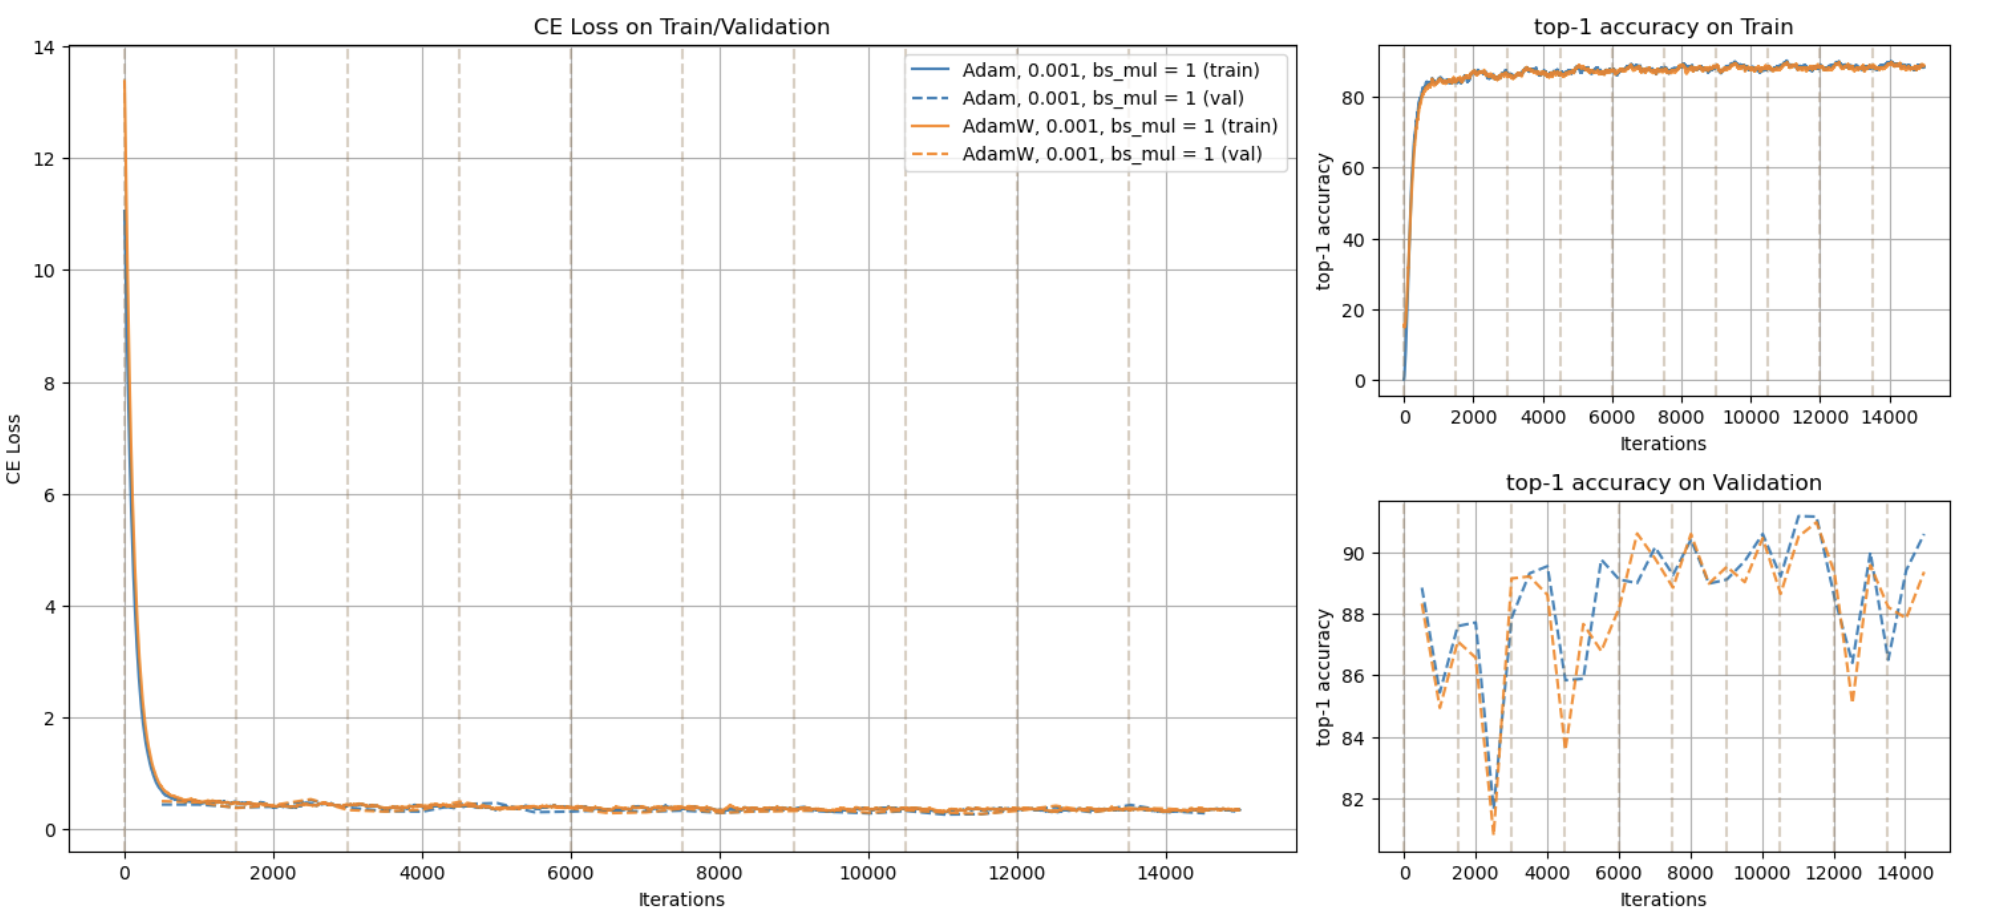
\includegraphics[width=0.5\linewidth]{./figures/sparse_cifar10_91.png}
    \caption{Лучший результат Sparse-CBM на CIFAR10.}
    \label{fig:sparse_best_cifar}
    \end{subfigure}
    \begin{subfigure}%[b]%{3.5cm}
    \centering
      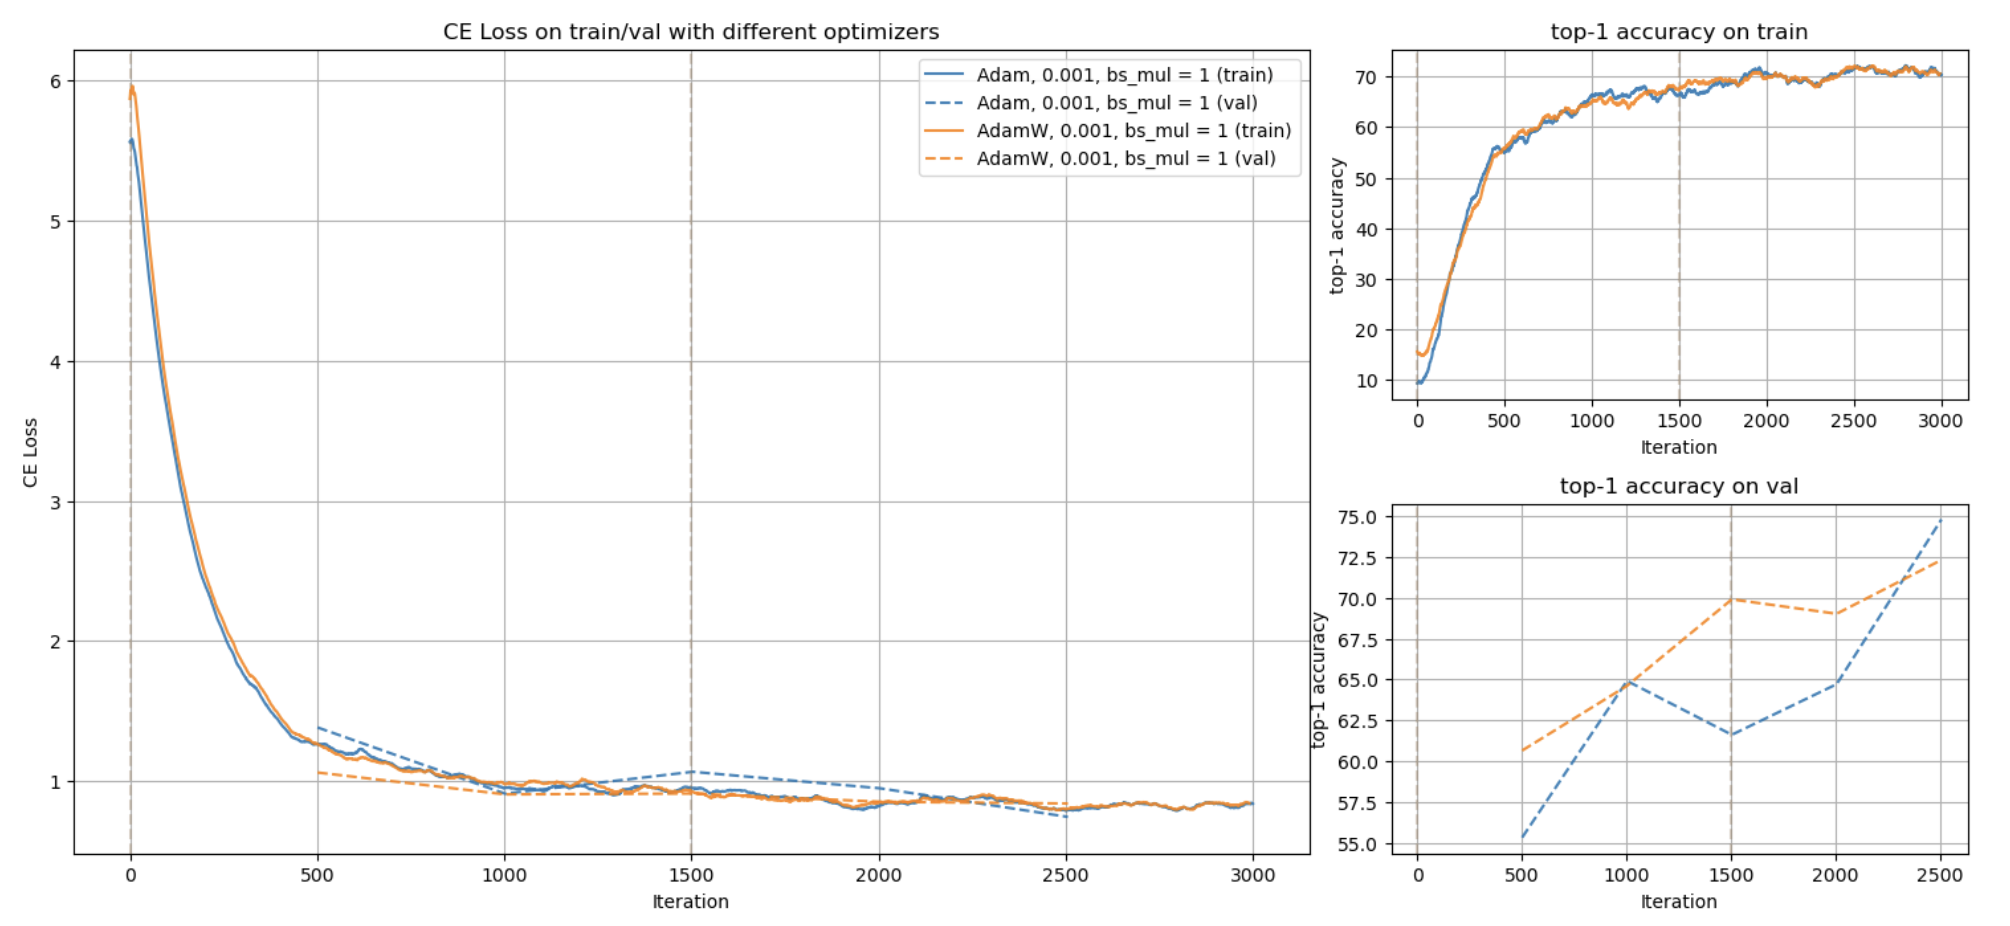
\includegraphics[width=0.5\linewidth]{./figures/sparse_imnet_71.png}
    \caption{Лучший результат Sparse-CBM на CUB200.}
    \label{fig:sparse_best_imnet}
    \end{subfigure}
    \begin{subfigure}%[b]%{3.5cm}
     \centering
  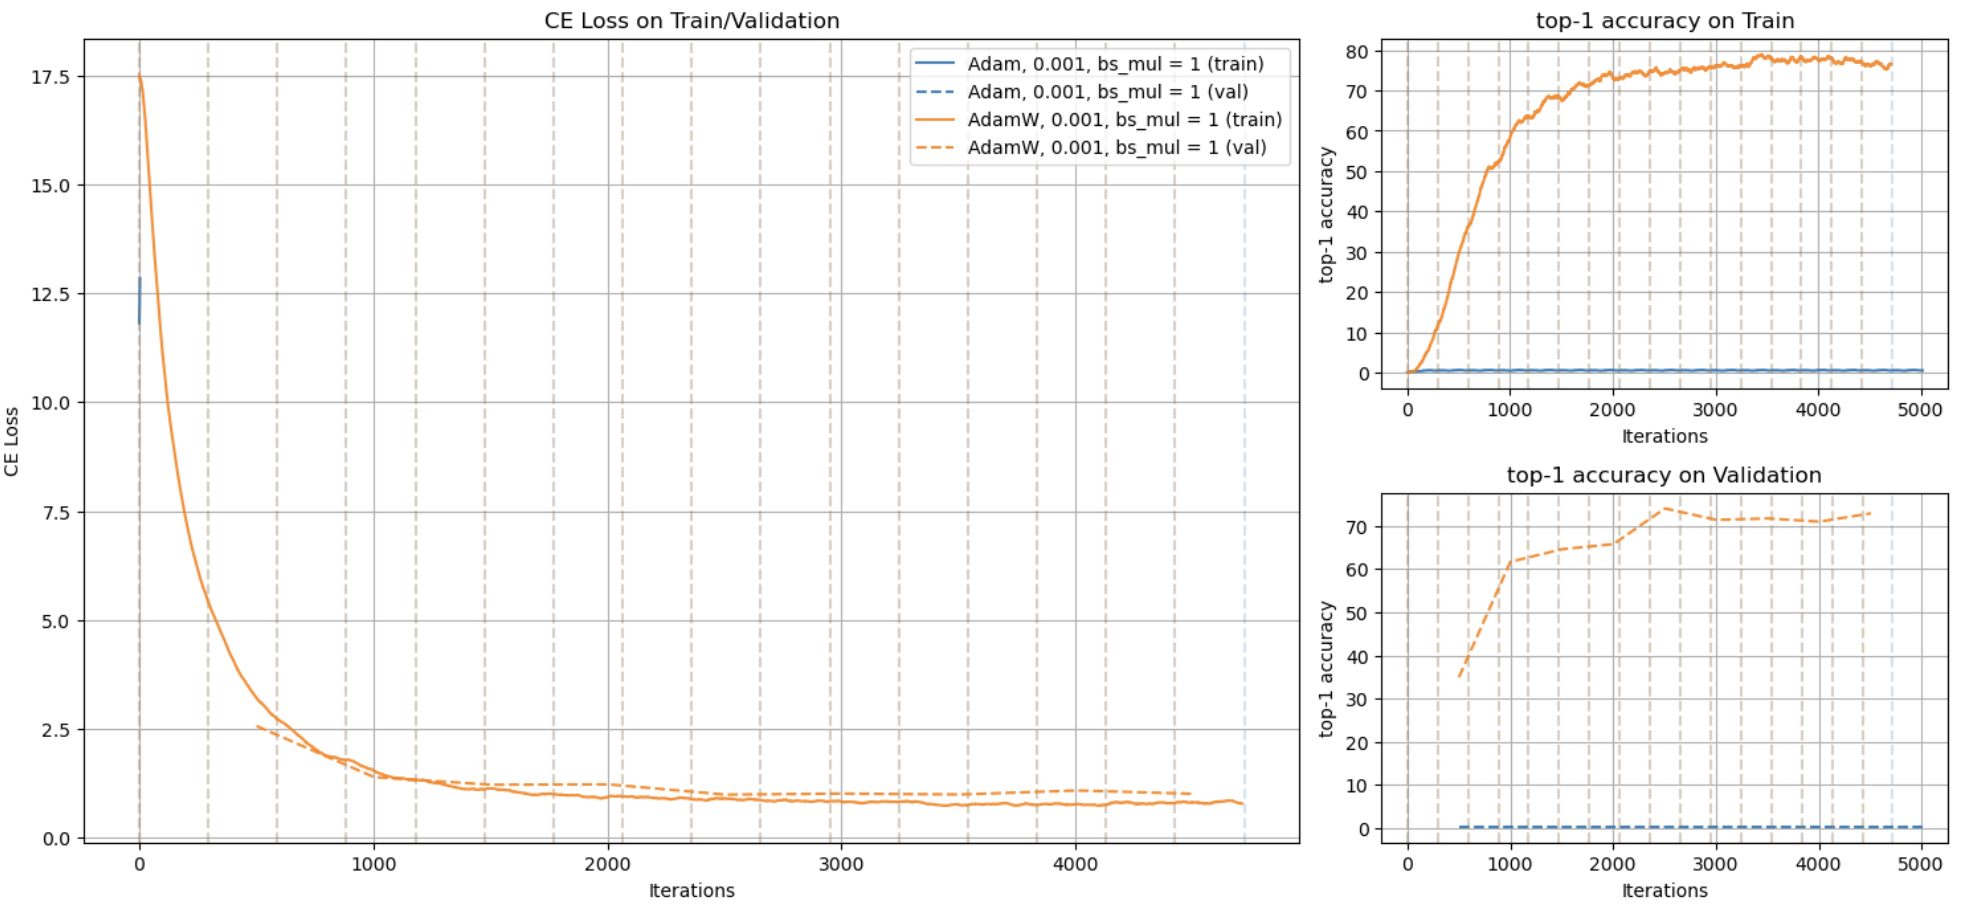
\includegraphics[width=0.5\linewidth]{./figures/sparse_cub_76.png}
    \caption{Лучший результат Sparse-CBM на ImageNet-1K.}
    \label{fig:sparse_best_cub}
    \end{subfigure}
    \caption{Обзор режима обучения с использованием разреженного CBM на нескольких наборах данных. Мы наблюдаем аналогичные кривые потерь при обучении на всех данных. Но для ImageNet обучение начинается с меньшей скорости обучения.}\label{fig:curves}
\end{figure}

\section{Дополнительные данные}

\begin{table}[h]
\caption{Конфигурации магистральных моделей. Пересечения указывают на размер модели с соответствующей конфигурацией.}
\label{tab:backbone_nets}
\begin{center}
\begin{small}
\begin{sc}
\begin{tabular}{lcccr}
\toprule
B/32 & L/14 & Dataset   \\
\midrule
 0.57GB & 1.63GB &  CIFAR10 \\
 0.58GB& 1.64GB & CIFAR100 \\
 0.68GB &  1.74GB & ImageNet \\
 0.58GB& 1.64GB & CUB200 \\
 0.61GB& 1.67GB & Places365 \\
\bottomrule
\end{tabular}
\end{sc}
\end{small}
\end{center}
\end{table}

\section{Визуализации}
\begin{figure}[ht]
\begin{center}
\centerline{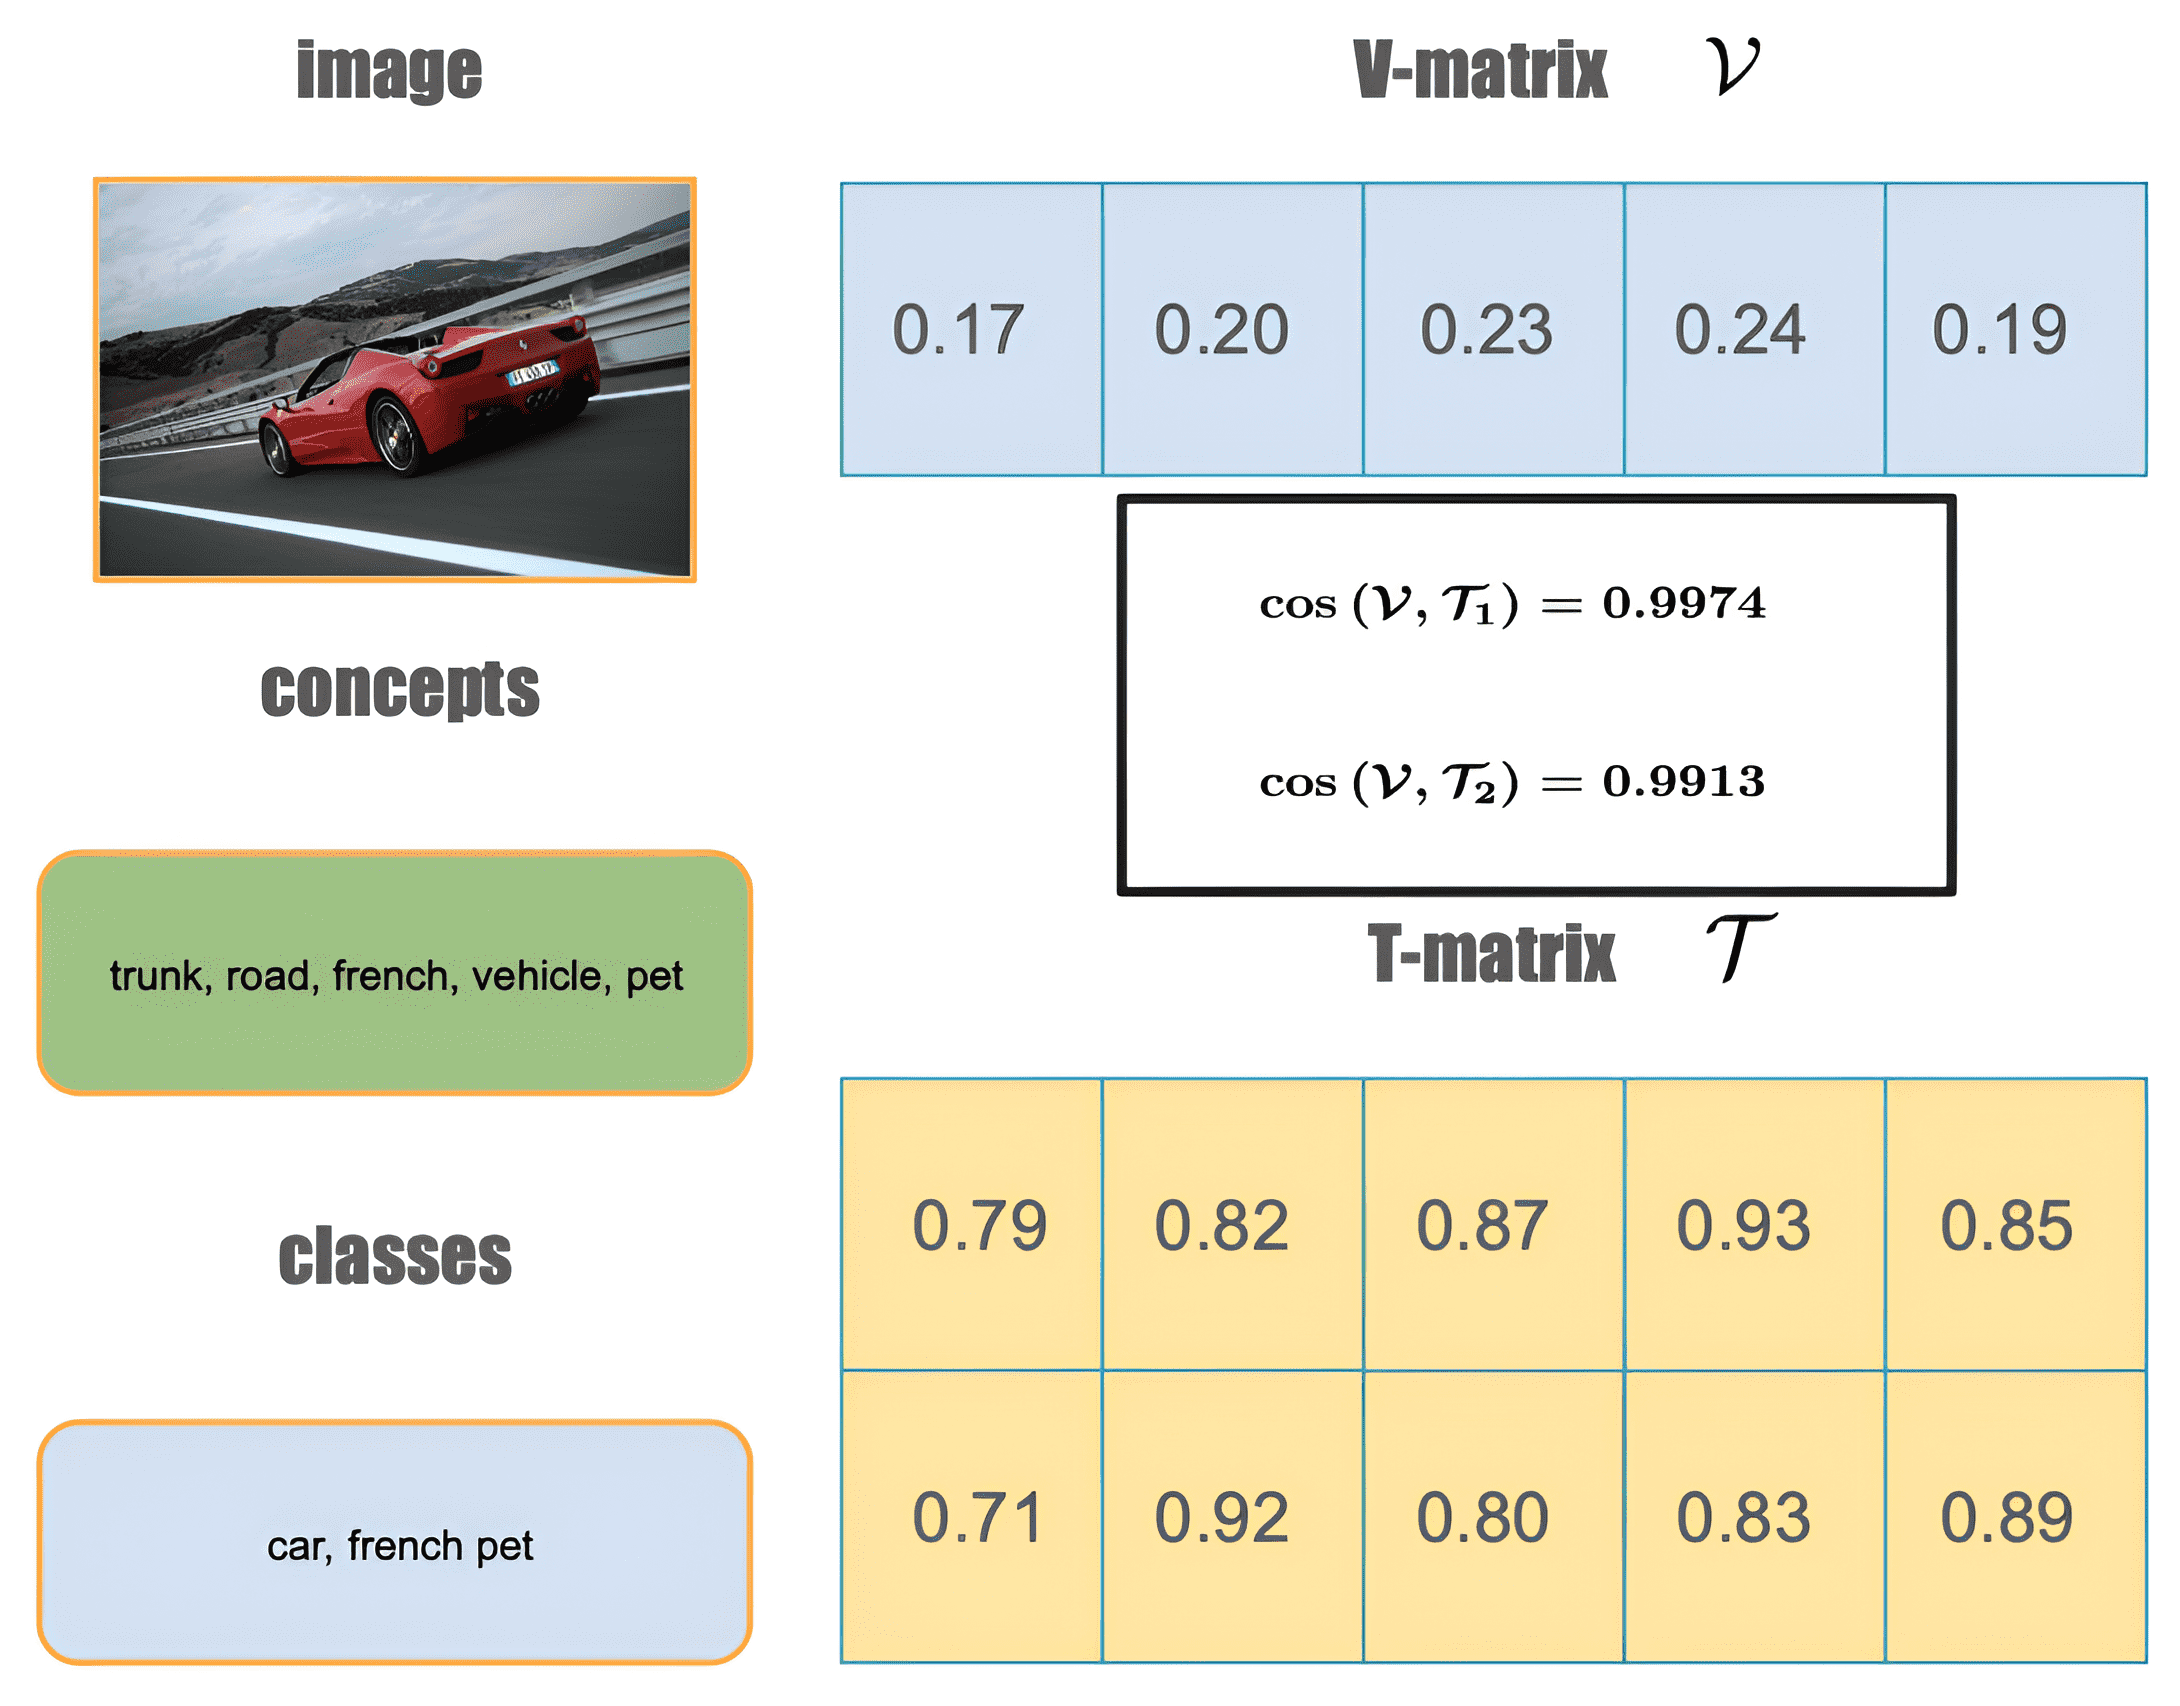
\includegraphics[width=0.5\columnwidth] {./figures/cms_example-compressed.png}} 
\caption{Визуализация Concept Matrix Search \textit{гипотезы} для простого случая 1 картинки, 5 концептов и 2 классов.}
\label{fig:cms_example}
\end{center}
\end{figure}

\subsection{Анализ латентного пространства CLIP}
В этом разделе мы представим дополнительные эксперименты с латентным пространством CLIP. Во-первых, используя CLIP, мы построили двумерную t-SNE карту вкраплений CIFAR10 вместе с их концептами и классами. Интересным результатом является то, что это пространство не просто разделено на два кластера: один соответствует текстовой модальности, а второй - визуальной, но и, если добавить проекцию случайных слов на t-SNE, мы наблюдаем ее пересечение с концептами. Соответствующий эксперимент представлен в \cref{fig:tsne}

С помощью метода кластеризации k-means мы строим различимые по CLIP кластеры (см. \cref{fig:kmeans}).

Важным моментом в t-SNE-визуализации является то, что латентное пространство CLIP-подобных моделей строго делится на два кластера: один соответствует вкраплениям изображений, а второй - текстовой модальности. Интуиция, лежащая в основе МД, подсказывает, что распределение модальностей должно полностью отличаться от того, что наблюдается в \cref{fig:tsne}. Действительно, для удобства интерпретации предполагается, что вкрапления изображений должны быть ближе к векторам соответствующих понятий и классов. Если это так, то простой алгоритм kNN сможет найти наиболее релевантные понятия, что в нашем случае неверно. Таким образом, мы выделяем нерешенную проблему построения моделей, которые будут изучать подобное латентное пространство сквозным образом.

\begin{figure}[h]
\begin{center}
\centerline{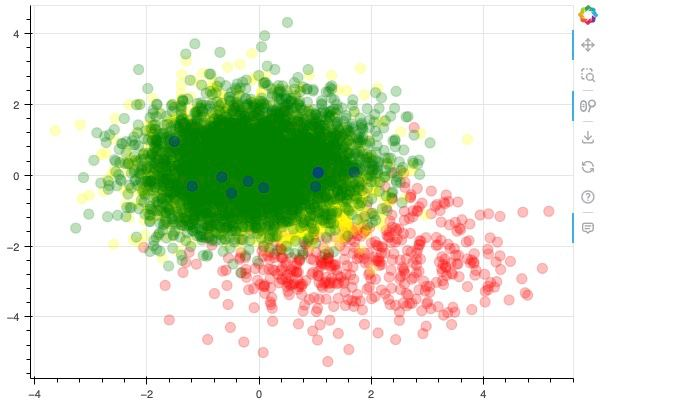
\includegraphics[width=0.5\columnwidth]{./figures/cifar10tsne.jpg}} 
\caption{Визуализация CIFAR10 t-SNE. Зеленые точки относятся к проекции понятий, синие - к классам, красные - к изображениям, а желтые - к случайным словам.}
\label{fig:tsne}
\end{center}
\end{figure}

\begin{figure}[t]%t
\begin{center}
\centerline{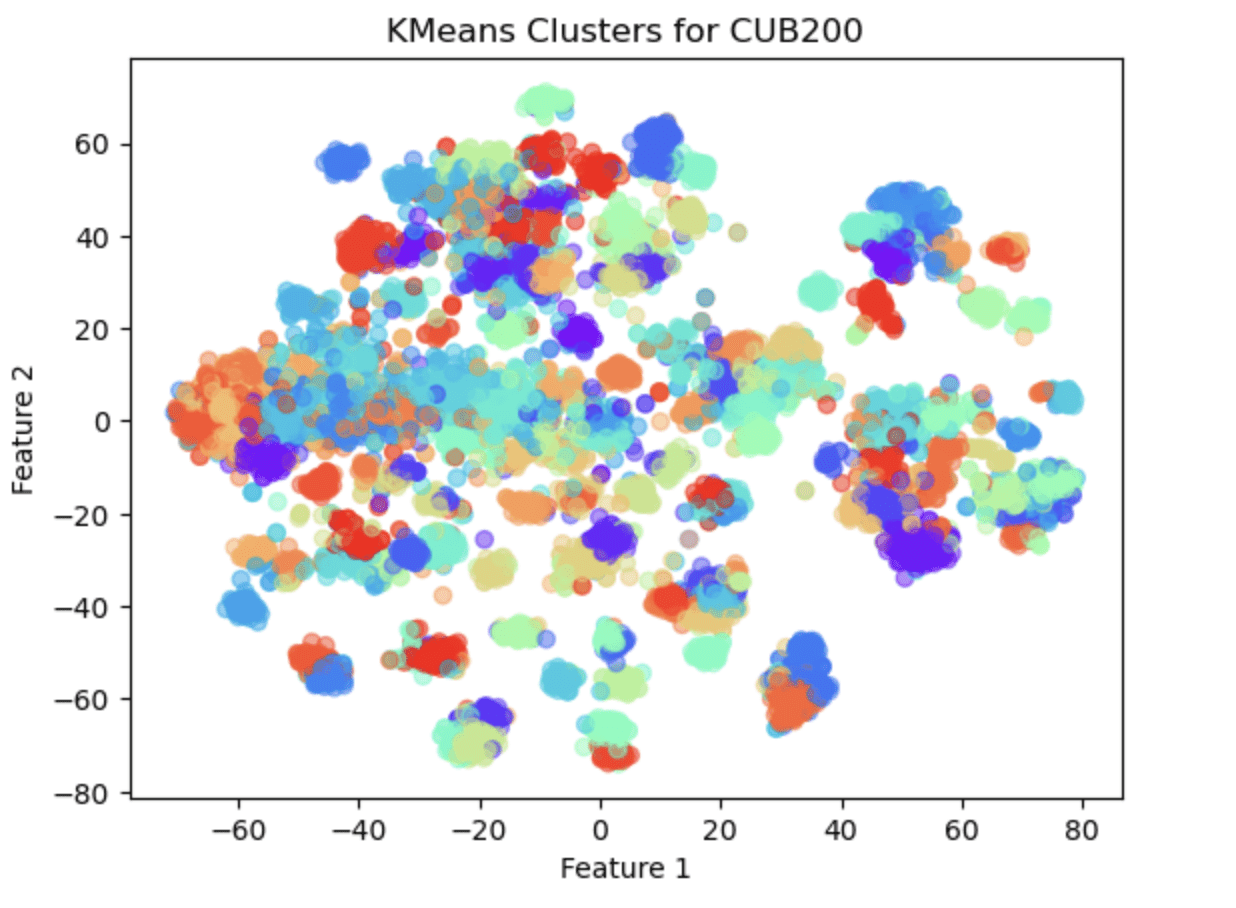
\includegraphics[width=\columnwidth]{./figures/cub_kmeans-compressed.png}} 
\caption{Визуализауия k-means кластеров эмбеддингов картинок из CUB200 полученных с помощью CLIP.}
\label{fig:kmeans}
\end{center}
\end{figure}


\subsection{Интерпретируемость концептов}
\label{sec:concepts_interpretability}
Мы сравниваем возможности интерпретации frawework с базовыми свойствами извлечения признаков CLIP на подмножествах изображений из наборов данных Places365, CUB200, CIFAR10 и ImageNet. Мы выбираем как базовые изображения для наглядности, так и сложные, с большим количеством внутренних деталей. Для CLIP-подобных моделей мы регистрируем топ-к (k=10) наивысших оценок точечного продукта, а для наших фреймворковых архитектур - результаты работы Concept Bottleneck Layer. Отметим, что дальнейшие результаты в \cref{fig:concepts_1,fig:concepts_2,fig:concepts_3,fig:concepts_4,fig:concepts_5,fig:concepts_6} проведены с использованием магистральной модели CLIP-ViT-L/14. Мы определенно наблюдаем распыление активаций с помощью как Sparse-, так и $\ell_1$-CBM. Также показано, что концептуальный слой Bottleneck Layer, обученный с контрастной целью, производит довольно схожие активации по сравнению с базовой моделью CLIP. В то же время итоговая точность становится выше при использовании разреженных и $\ell_1$-моделей, что говорит о превосходстве методов, разрежающих внутренние слои модели.

В данной работе мы не приводим интерпретируемые матрицы поиска концептов, поскольку этот подход к классификации с узкими местами концептов не модифицирует базовую модель CLIP, поэтому она обладает теми же свойствами, что и \cref{fig:concepts_1,fig:concepts_2,fig:concepts_3,fig:concepts_4,fig:concepts_5,fig:concepts_6} (a).
\begin{figure}[h] %ht!
\centering
   \begin{subfigure}%[b]%{3.5cm}
     \centering
    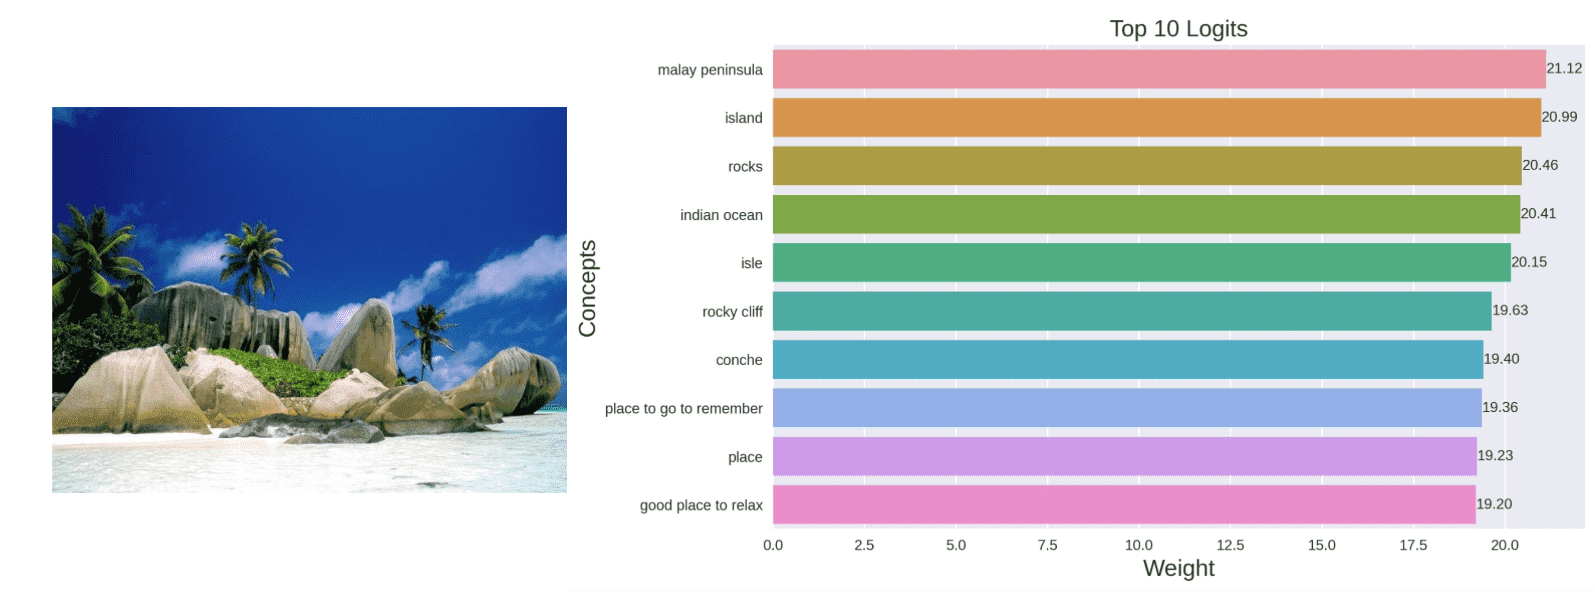
\includegraphics[width=0.75\linewidth]{./figures/clip_im_1-compressed.png}
    % \caption{Концепты, извлекаемые с помощью CLIP.}
    \\
    (a) Концепты, извлекаемые с помощью CLIP.
    % \label{fig:clip_im_1}
    \end{subfigure}
    \begin{subfigure}%[b]%{3.5cm}
    \centering
      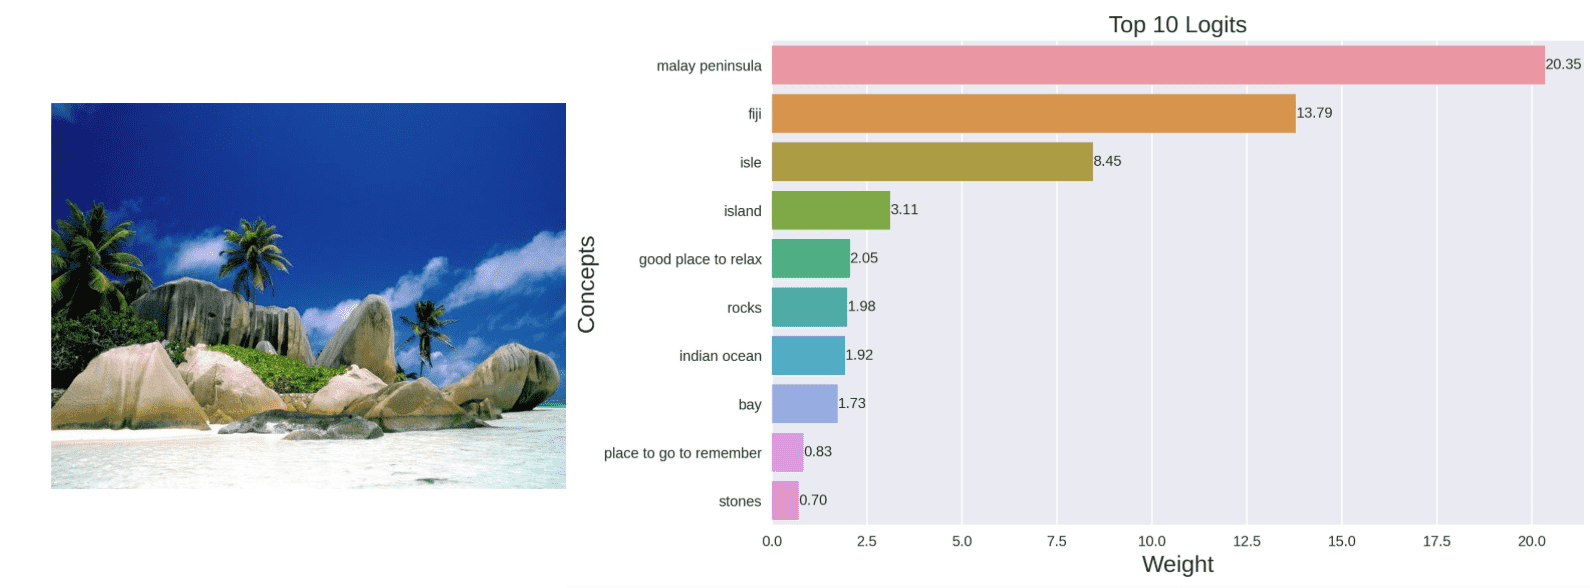
\includegraphics[width=0.75\linewidth]{./figures/sparse_im_1-compressed.png}
    % \caption{Концепты, извлекаемые с помощью Sparse-CBM.}
    \\
    (b) Концепты, извлекаемые с помощью Sparse-CBM.
    % \label{fig:sparse_im_1}
    \end{subfigure}
    \begin{subfigure}%[b]%{3.5cm}
     \centering
  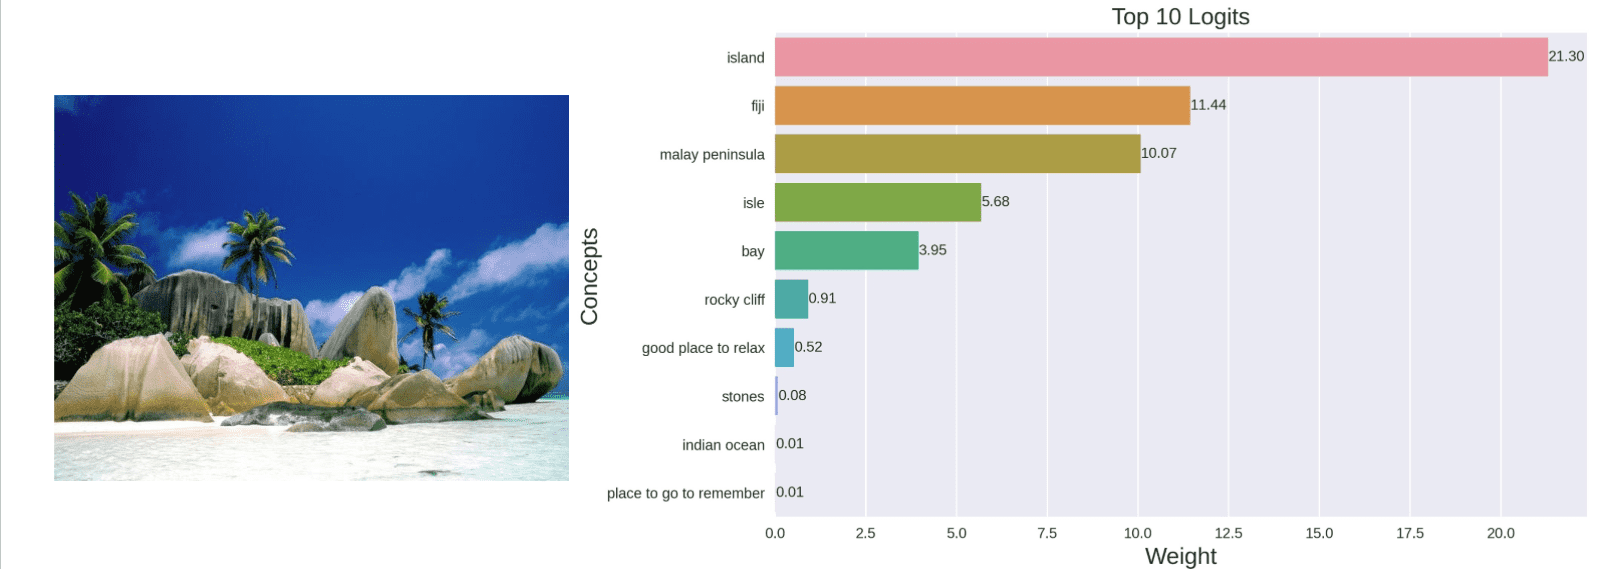
\includegraphics[width=0.75\linewidth]{./figures/l1_im1-compressed.png}
    % \caption{Концепты, извлекаемые с помощью $\ell_1$-CBM.}
    \\
    (c) Концепты, извлекаемые с помощью $\ell_1$-CBM.
    % \label{fig:l1_im_1}
    \end{subfigure}
        \begin{subfigure}%[b]%{3.5cm}
     \centering
  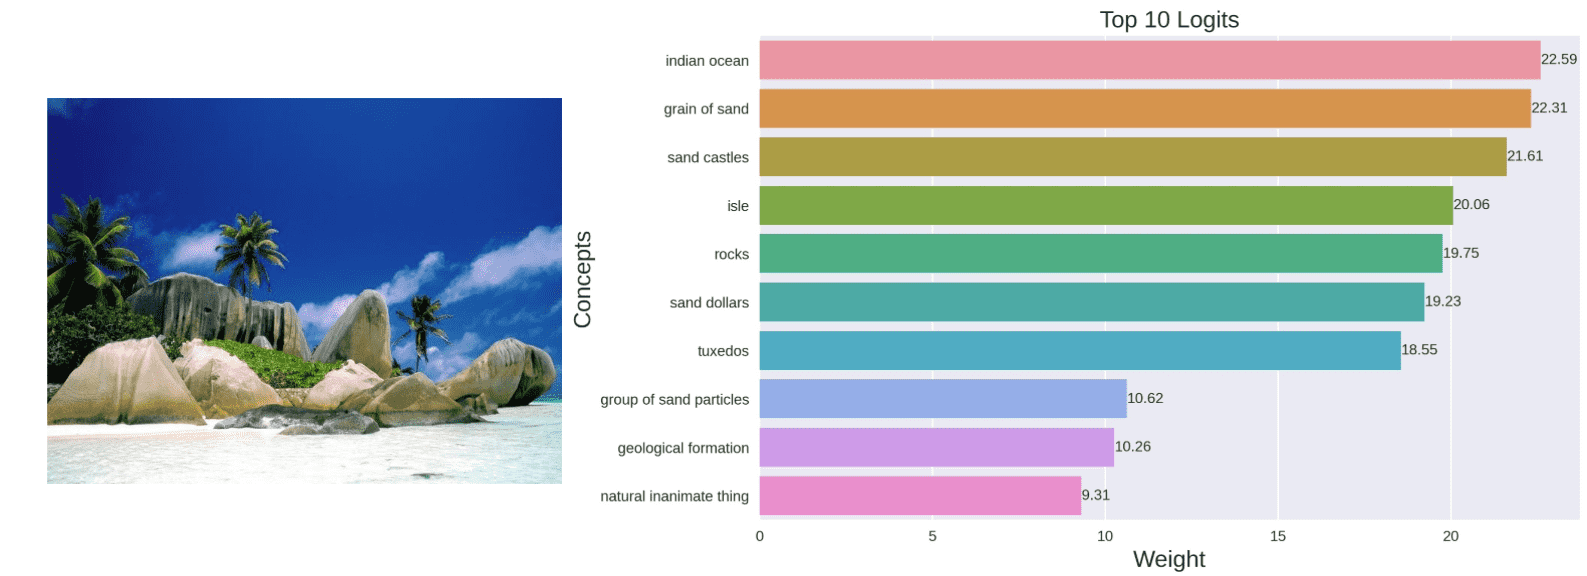
\includegraphics[width=0.75\linewidth]{./figures/contr_im_1-compressed.png}
    % \caption{Концепты, извлекаемые с помощью Contrastive-CBM.}
    \\
    (d) Концепты, извлекаемые с помощью Contrastive-CBM.
    % \label{fig:contr_im_1}
    \end{subfigure}
    \caption{Концепты, извлекаемые с помощью моделей, обученных на Places365.}
    \label{fig:concepts_1}
\end{figure}

\begin{figure}[h] %ht!
\centering
   \begin{subfigure}%[b]%{3.5cm}
     \centering
    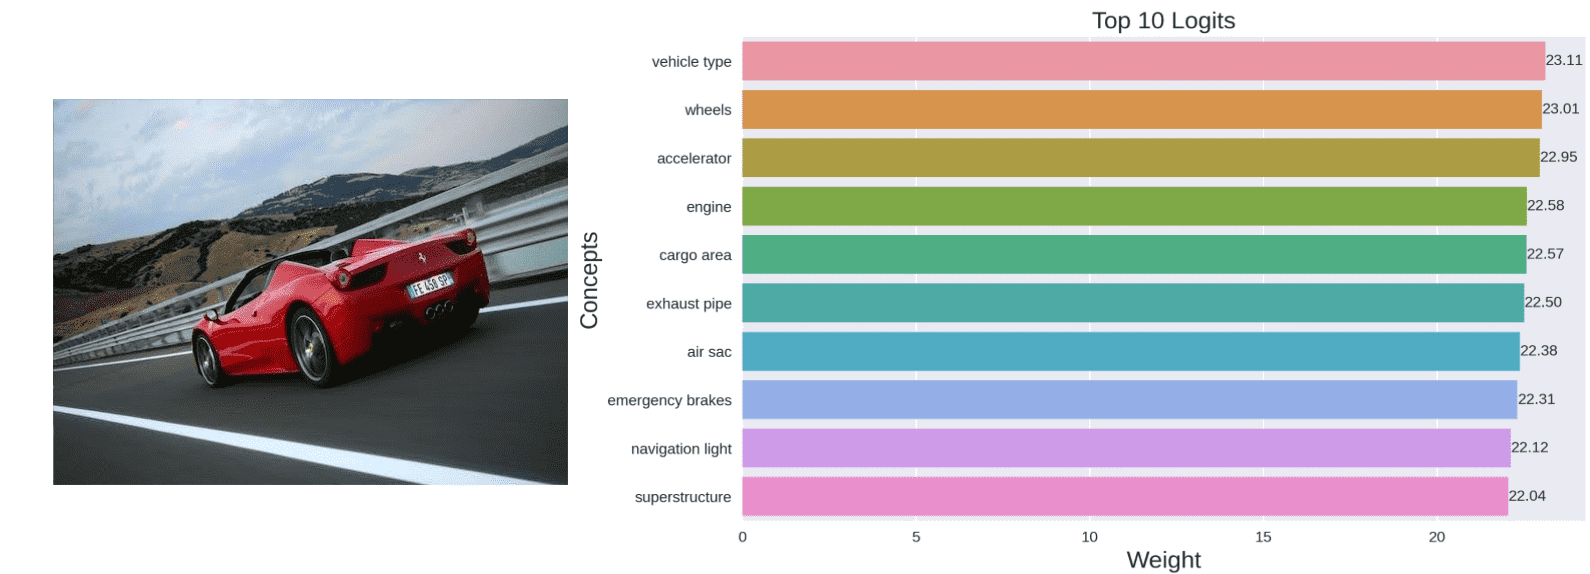
\includegraphics[width=0.75\linewidth]{./figures/clip_im_2-compressed.png}
    % \caption{Концепты, извлекаемые с помощью CLIP.}
    \\
    (a) Концепты, извлекаемые с помощью CLIP.
    % \label{fig:clip_im_2}
    \end{subfigure}
    \begin{subfigure}%[b]%{3.5cm}
    \centering
      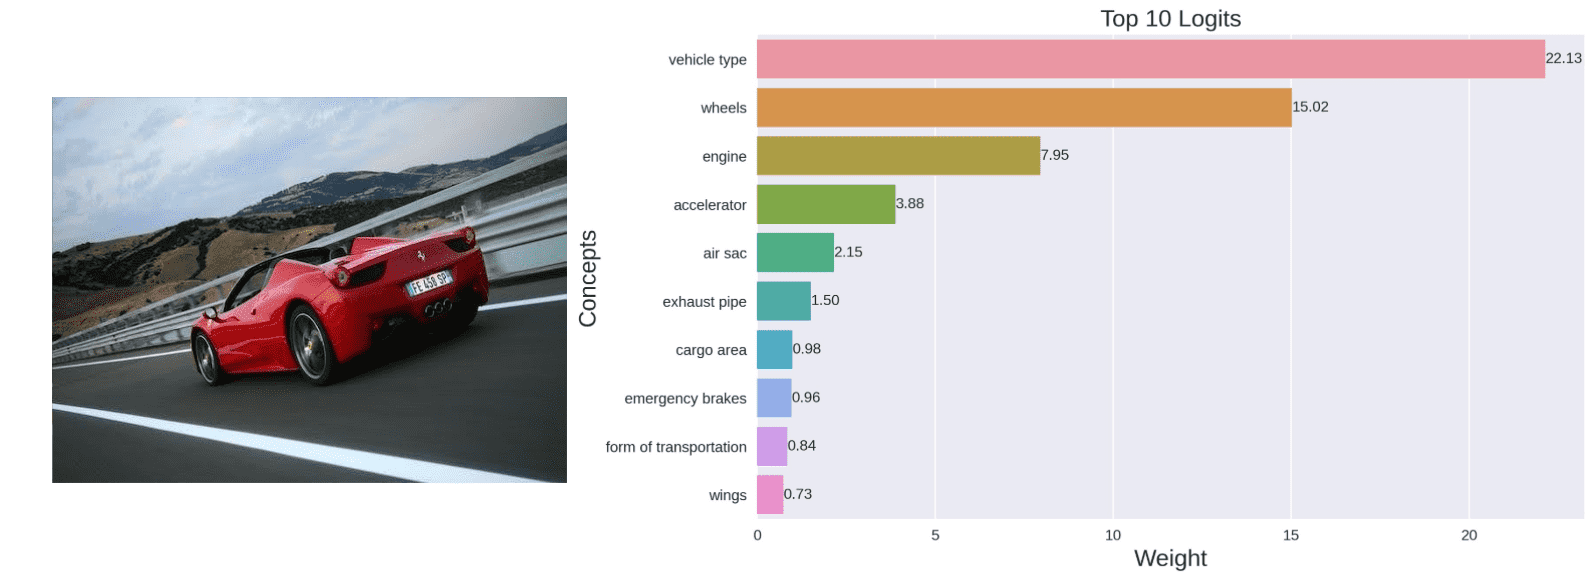
\includegraphics[width=0.75\linewidth]{./figures/sparse_im_2-compressed.png}
    % \caption{Концепты, извлекаемые с помощью Sparse-CBM.}
    \\
    (b) Концепты, извлекаемые с помощью sparse-CBM.
    % \label{fig:sparse_im_2}
    \end{subfigure}
    \begin{subfigure}%[b]%{3.5cm}
     \centering
  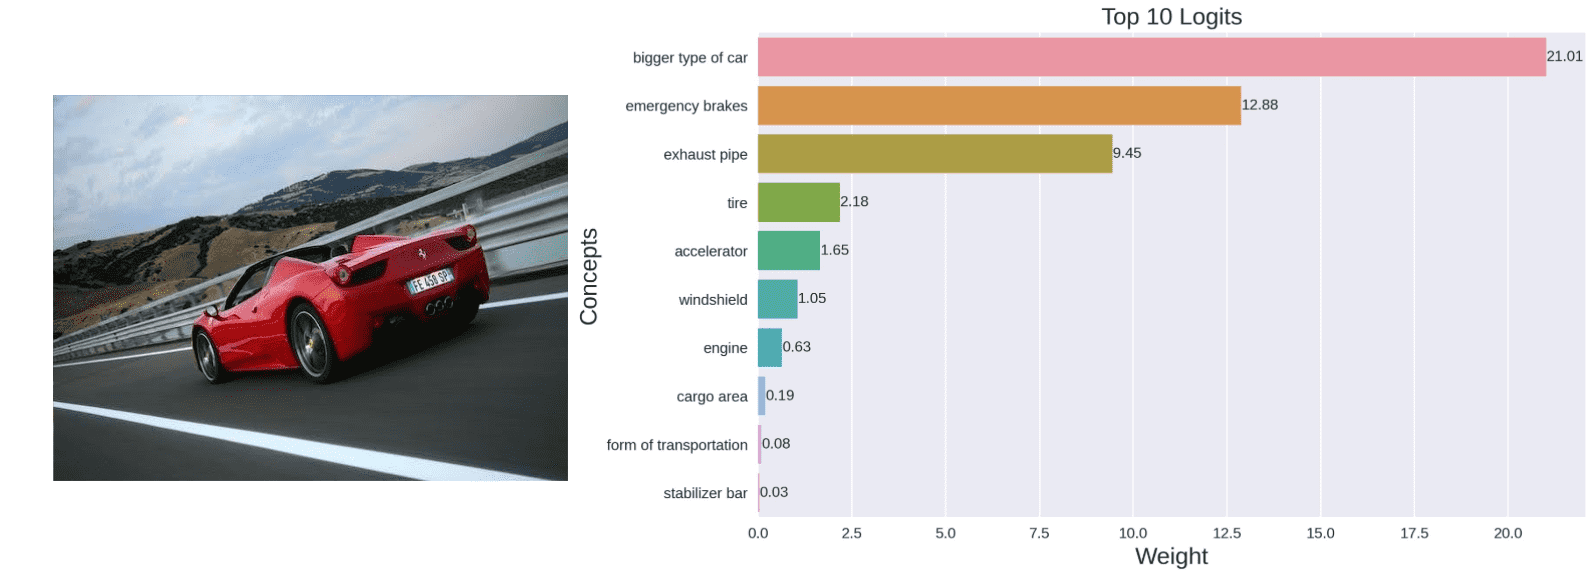
\includegraphics[width=0.75\linewidth]{./figures/l1_im_2-compressed.png}
    % \caption{Концепты, извлекаемые с помощью $\ell_1$-CBM.}
    \\
    (c) Концепты, извлекаемые с помощью $\ell_1$-CBM.
    % \label{fig:l1_im_2}
    \end{subfigure}
        \begin{subfigure}%[b]%{3.5cm}
     \centering
  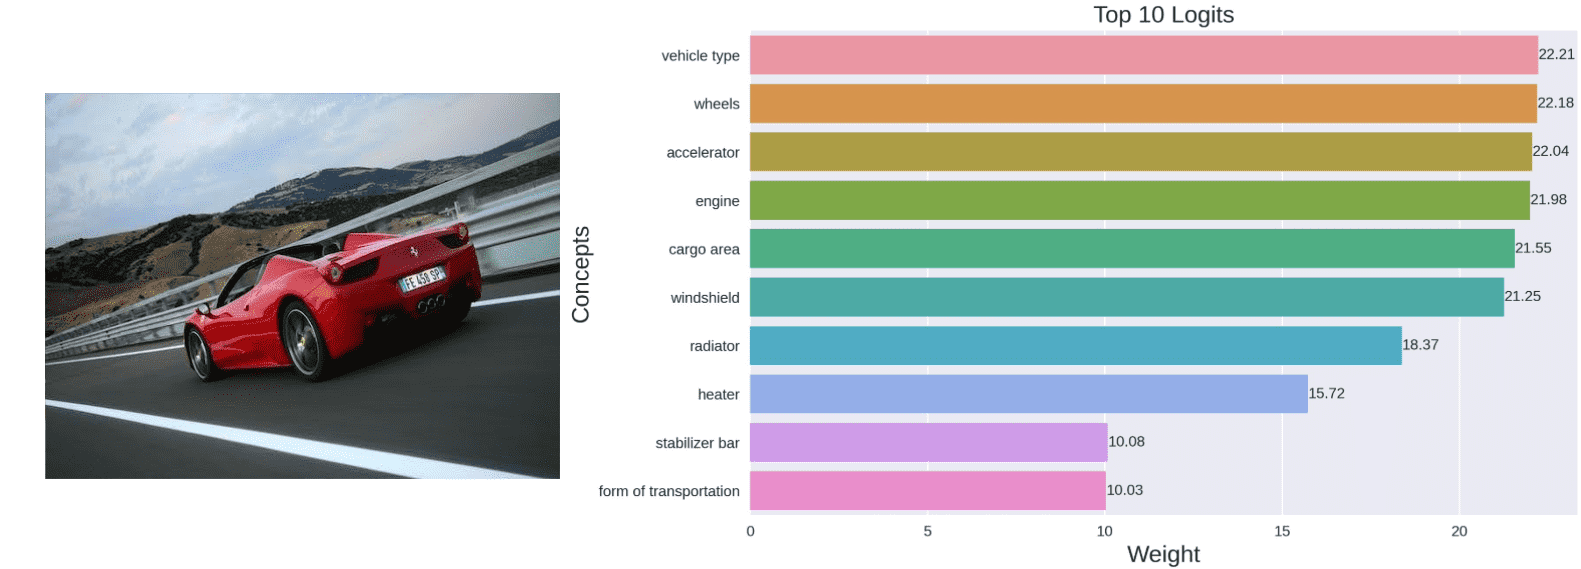
\includegraphics[width=0.75\linewidth]{./figures/contr_im_2-compressed.png}
    % \caption{Концепты, извлекаемые с помощью Contrastive-CBM.}
    \\
    (d) Концепты, извлекаемые с помощью Contrastive-CBM.
    % \label{fig:contr_im_2}
    \end{subfigure}
    \caption{Концепты, извлекаемые с помощью моделей, обученных на CIFAR10.}
    \label{fig:concepts_2}
\end{figure}

\begin{figure}[h] %ht!
\centering
   \begin{subfigure}%[b]%{3.5cm}
     \centering
    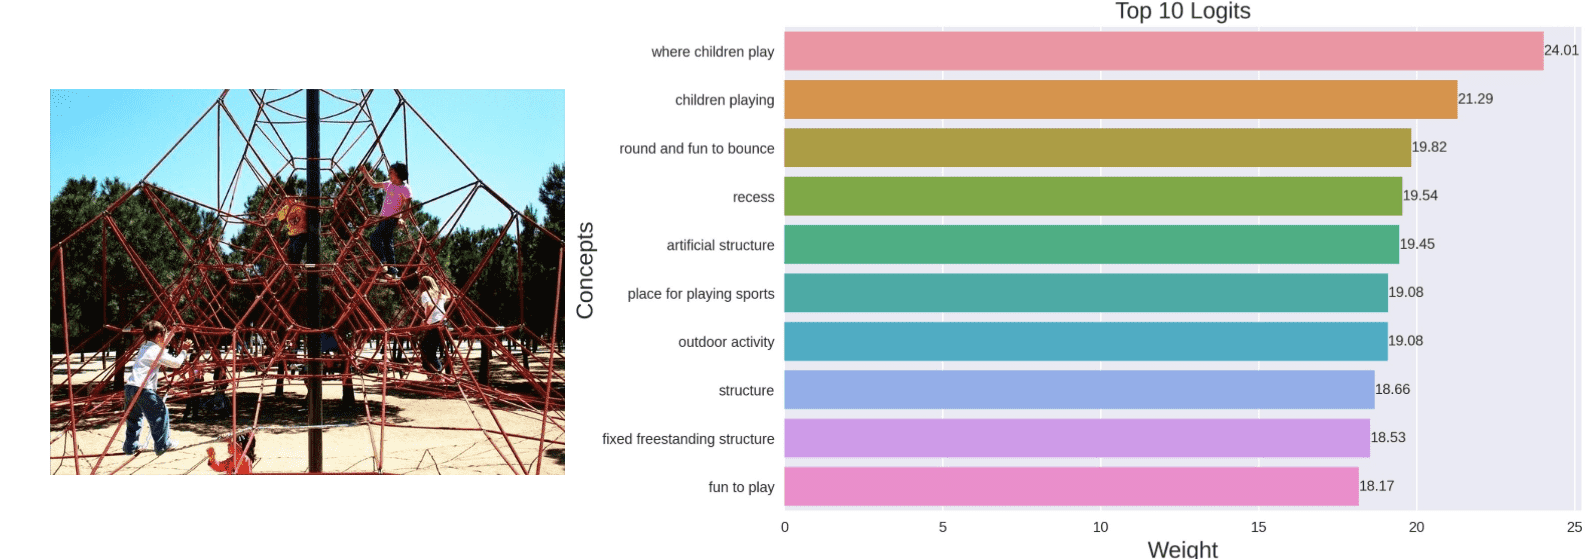
\includegraphics[width=0.75\linewidth]{./figures/clip_im_3-compressed.png}
    % \caption{Концепты, извлекаемые с помощью CLIP.}
    \\
    (a) Концепты, извлекаемые с помощью CLIP.
    % \label{fig:clip_im_3}
    \end{subfigure}
    \begin{subfigure}%[b]%{3.5cm}
    \centering
      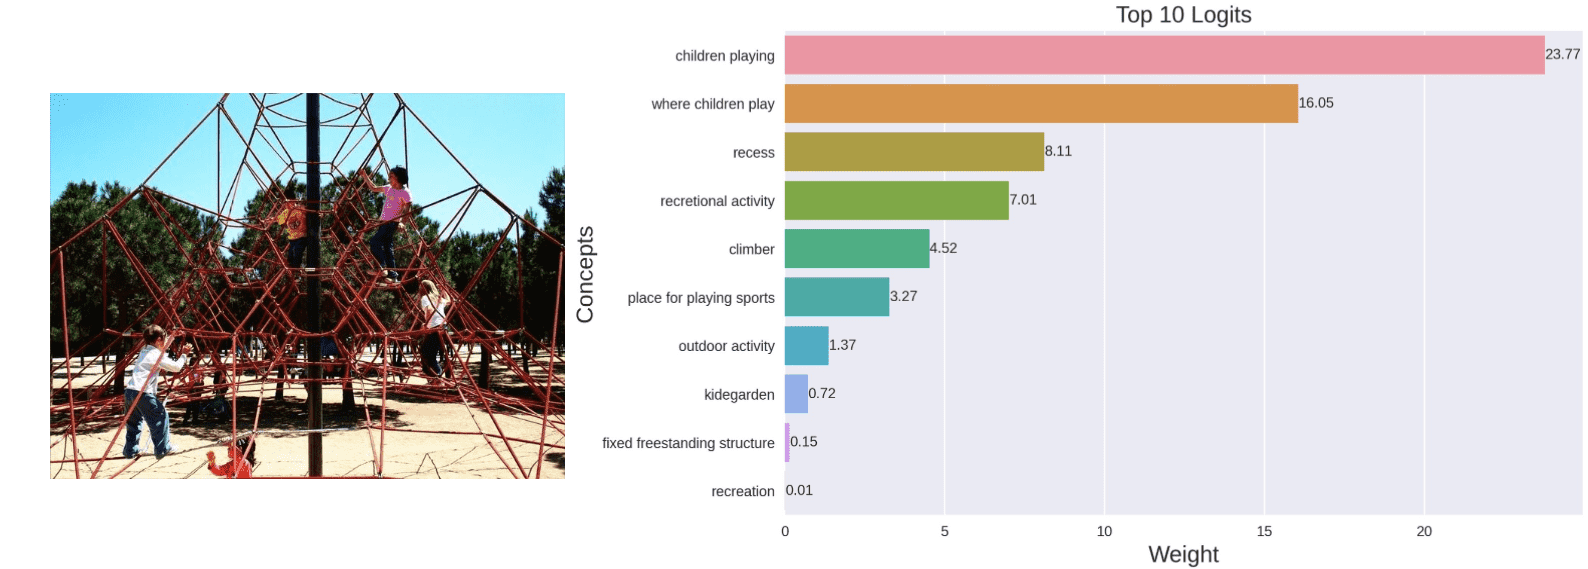
\includegraphics[width=0.75\linewidth]{./figures/sparse_im_3-compressed.png}
    % \caption{Концепты, извлекаемые с помощью Sparse-CBM.}
    \\
    (b) Концепты, извлекаемые с помощью Sparse-CBM.
    % \label{fig:sparse_im_3}
    \end{subfigure}
    \begin{subfigure}%[b]%{3.5cm}
     \centering
  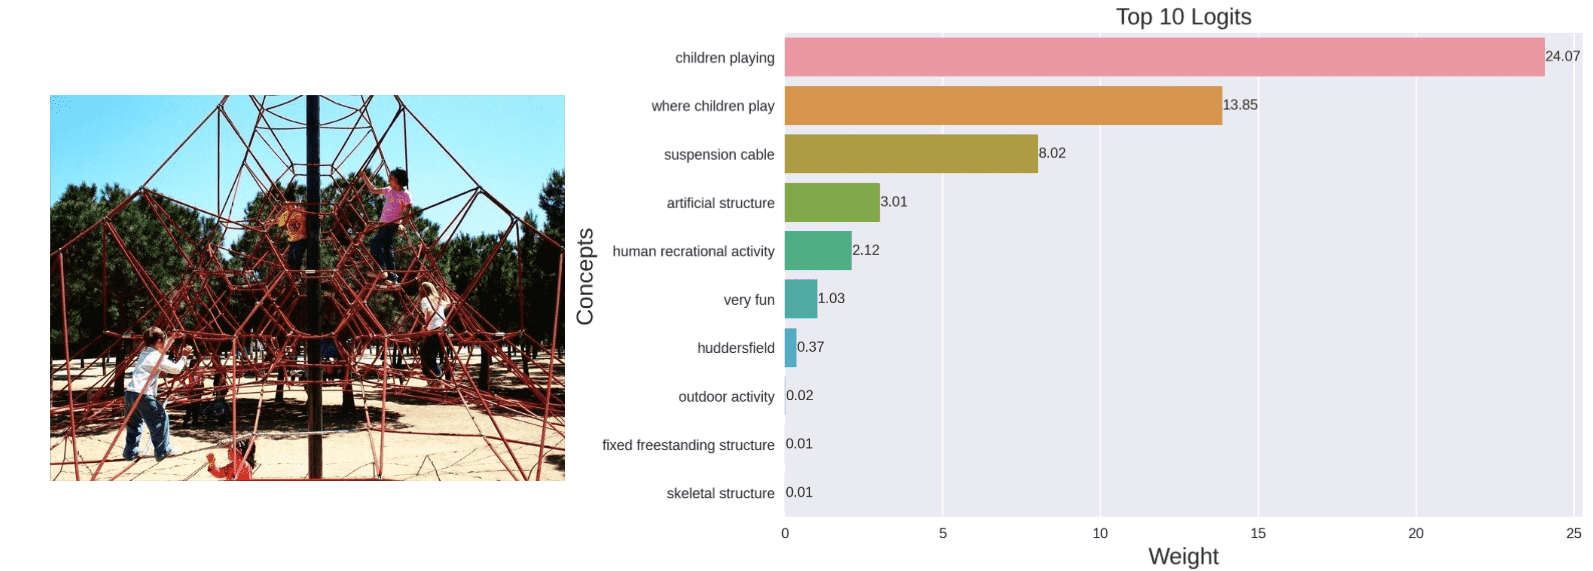
\includegraphics[width=0.75\linewidth]{./figures/l1_im_3-compressed.png}
    % \caption{Концепты, извлекаемые с помощью $\ell_1$-CBM.}
    \\
    (c) Концепты, извлекаемые с помощью $\ell_1$-CBM.
    % \label{fig:l1_im_3}
    \end{subfigure}
        \begin{subfigure}%[b]%{3.5cm}
     \centering
  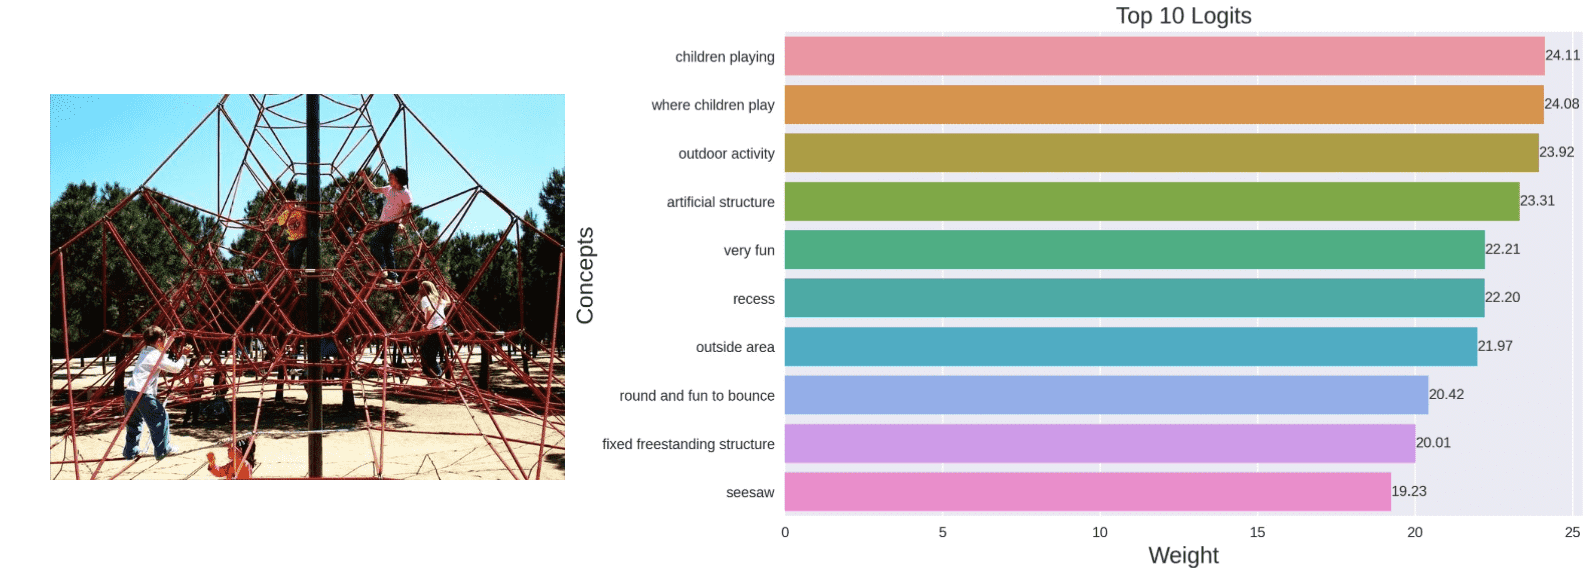
\includegraphics[width=0.75\linewidth]{./figures/contr_im_3-compressed.png}
    % \caption{Концепты, извлекаемые с помощью Contrastive-CBM.}
    \\
    (d) Концепты, извлекаемые с помощью Contrastive-CBM.
    % \label{fig:contr_im_3}
    \end{subfigure}
    \caption{Концепты, извлекаемые с помощью моделей, обученных на Places365.}
    \label{fig:concepts_3}
\end{figure}

\begin{figure}[h] %ht!
\centering
   \begin{subfigure}%[b]%{3.5cm}
     \centering
    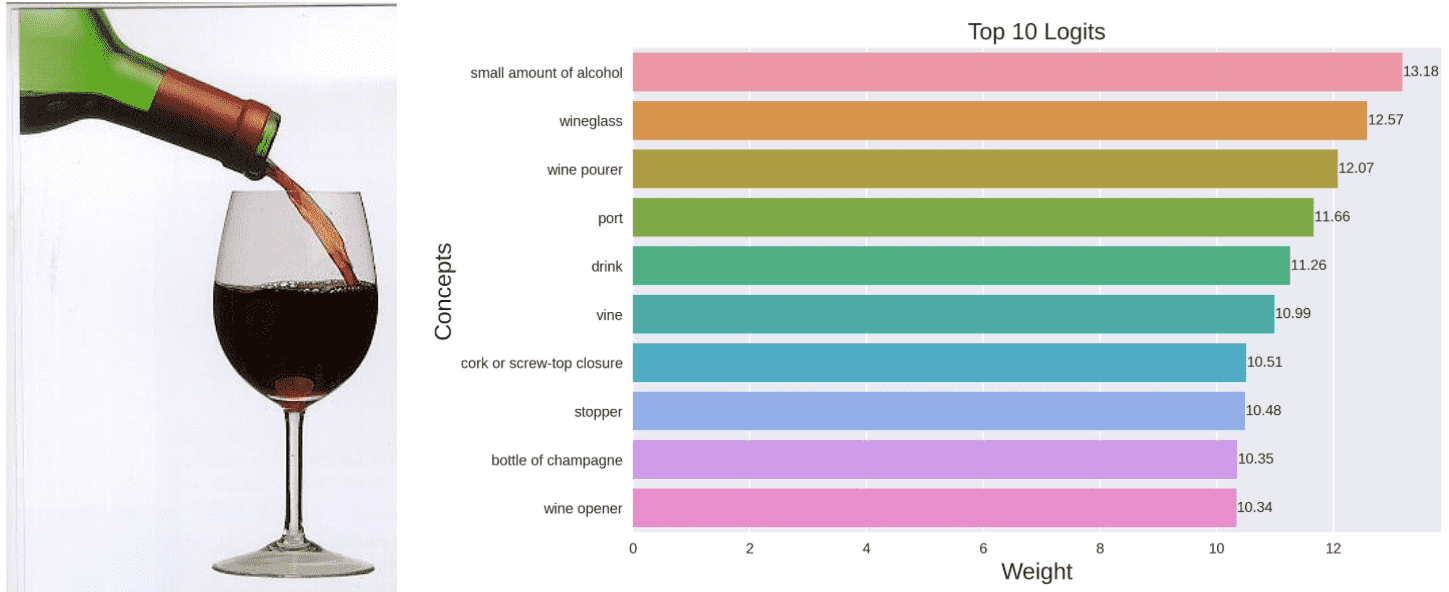
\includegraphics[width=0.65\linewidth]{./figures/clip_im_4-compressed.png}
    % \caption{Концепты, извлекаемые с помощью CLIP.}
    \\
    (a) Концепты, извлекаемые с помощью CLIP.
    % \label{fig:clip_im_4}
    \end{subfigure}
    \begin{subfigure}%[b]%{3.5cm}
    \centering
      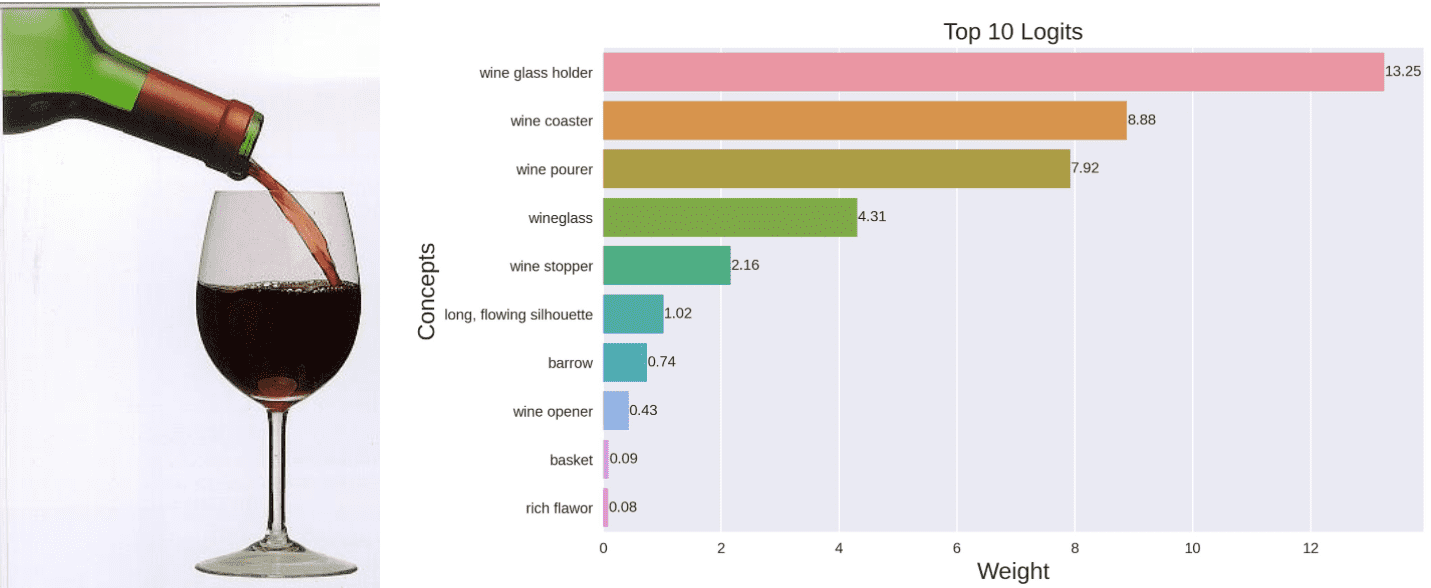
\includegraphics[width=0.65\linewidth]{./figures/sparse_im_4-compressed.png}
    % \caption{Концепты, извлекаемые с помощью Sparse-CBM.}
    \\
    (b) Концепты, извлекаемые с помощью Sparse-CBM.
    % \label{fig:sparse_im_4}
    \end{subfigure}
    \begin{subfigure}%[b]%{3.5cm}
     \centering
  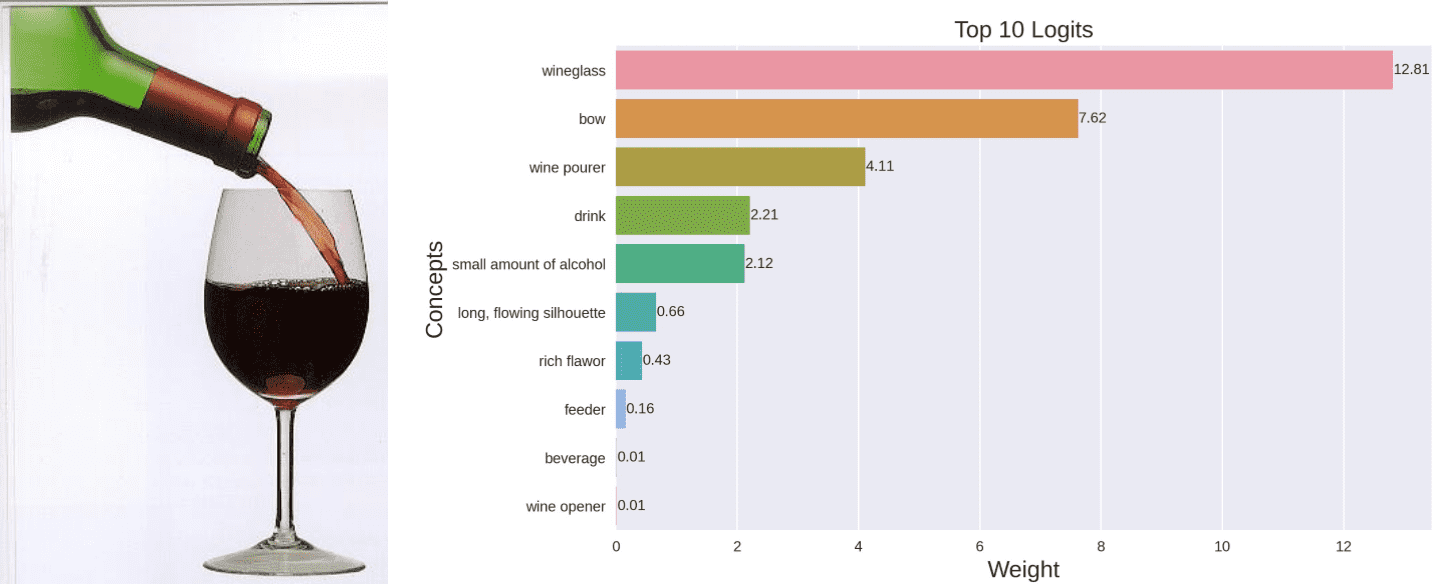
\includegraphics[width=0.65\linewidth]{./figures/l1_im_4-compressed.png}
    % \caption{Концепты, извлекаемые с помощью $\ell_1$-CBM.}
    \\
    (c) Концепты, извлекаемые с помощью $\ell_1$-CBM.
    % \label{fig:l1_im_4}
    \end{subfigure}
        \begin{subfigure}%[b]%{3.5cm}
     \centering
  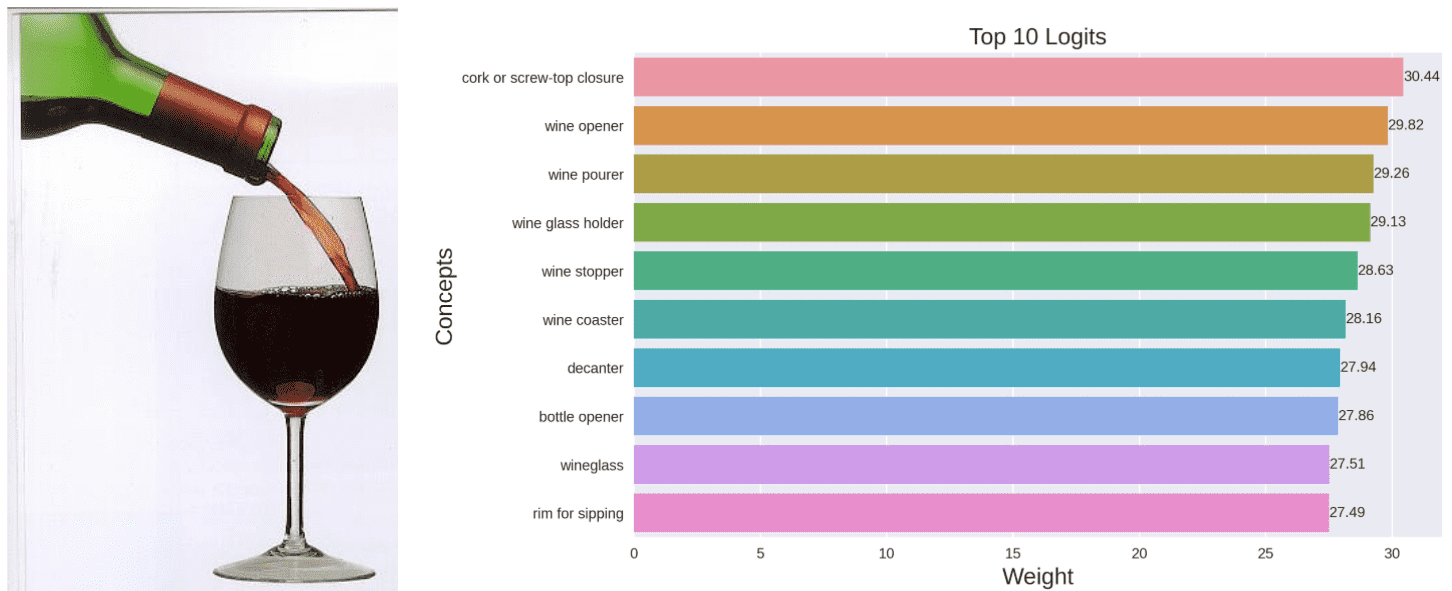
\includegraphics[width=0.65\linewidth]{./figures/contr_im_4-compressed.png}
    % \caption{Концепты, извлекаемые с помощью Contrastive-CBM.}
    \\
    (d) Концепты, извлекаемые с помощью Contrastive-CBM.
    % \label{fig:contr_im_4}
    \end{subfigure}
    \caption{Концепты, извлекаемые с помощью моделей, обученных на ImageNet.}
    \label{fig:concepts_4}
\end{figure}

\begin{figure}[h] %ht!
\centering
   \begin{subfigure}%[b]%{3.5cm}
     \centering
    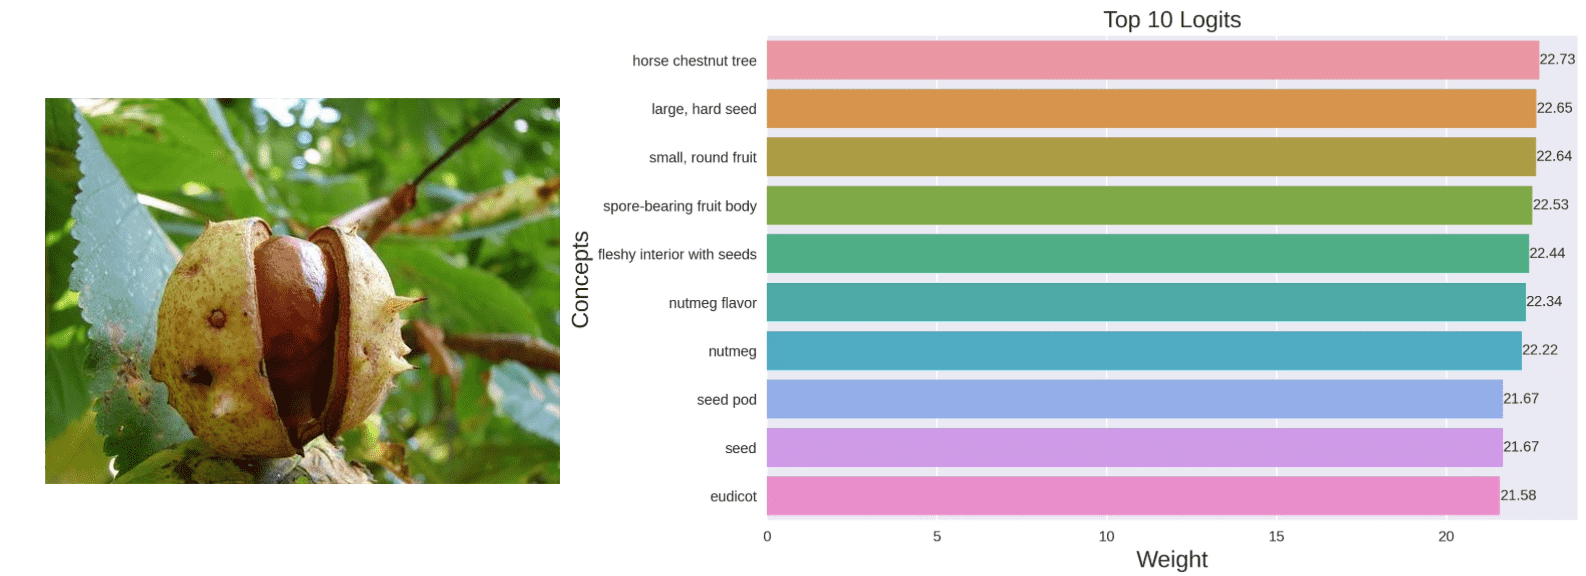
\includegraphics[width=0.7\linewidth]{./figures/clip_im_5-compressed.png}
    % \caption{Концепты, извлекаемые с помощью CLIP.}
    \\
    (a) Концепты, извлекаемые с помощью CLIP.
    % \label{fig:clip_im_5}
    \end{subfigure}
    \begin{subfigure}%[b]%{3.5cm}
    \centering
      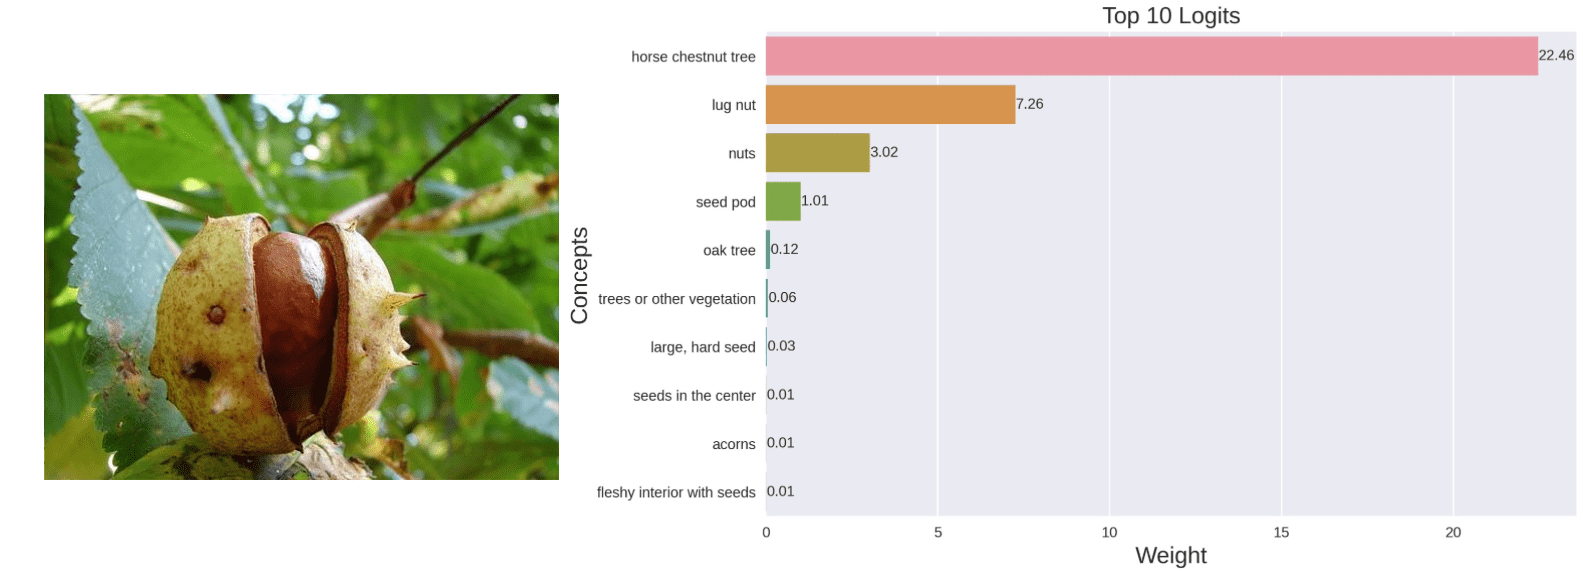
\includegraphics[width=0.7\linewidth]{./figures/sparse_im_5-compressed.png}
    % \caption{Концепты, извлекаемые с помощью Sparse-CBM.}
    \\
    (b) Концепты, извлекаемые с помощью Sparse-CBM.
    % \label{fig:sparse_im_5}
    \end{subfigure}
    \begin{subfigure}%[b]%{3.5cm}
     \centering
  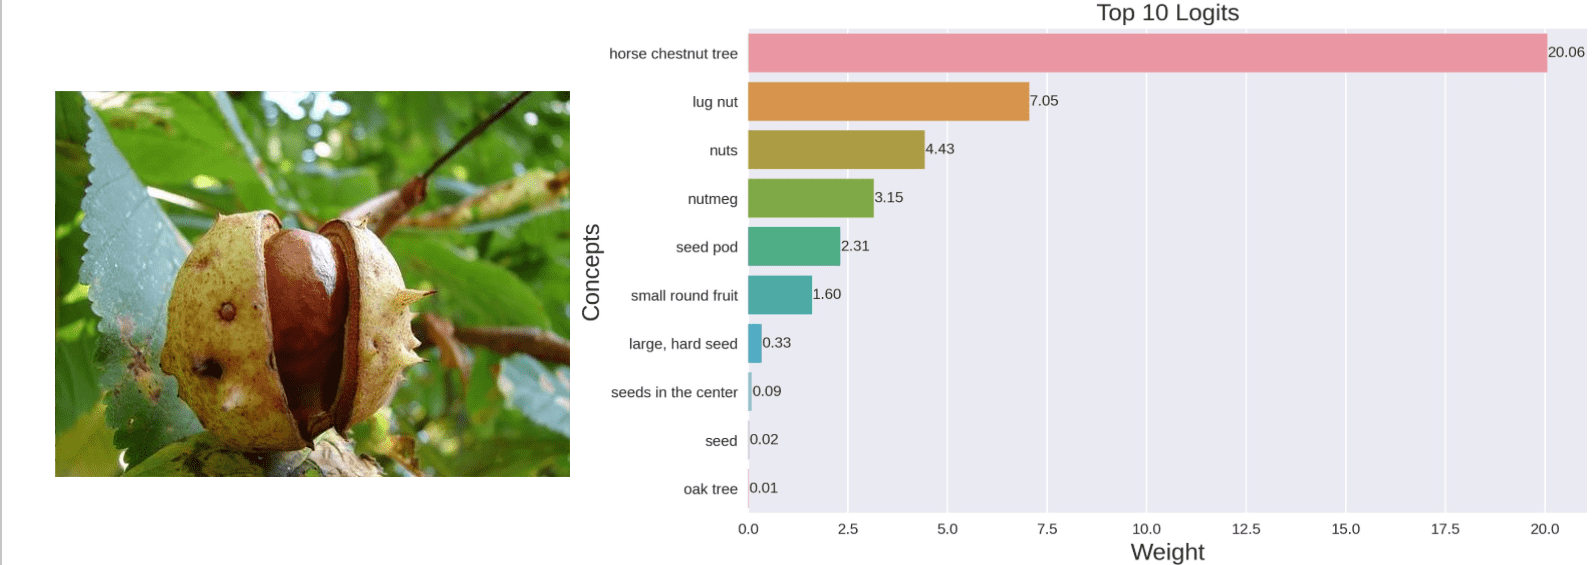
\includegraphics[width=0.75\linewidth]{./figures/l1_im_5-compressed.png}
    % \caption{Концепты, извлекаемые с помощью $\ell_1$-CBM.}
    \\
    (c) Концепты, извлекаемые с помощью $\ell_1$-CBM.
    % \label{fig:l1_im_5}
    \end{subfigure}
        \begin{subfigure}%[b]%{3.5cm}
     \centering
  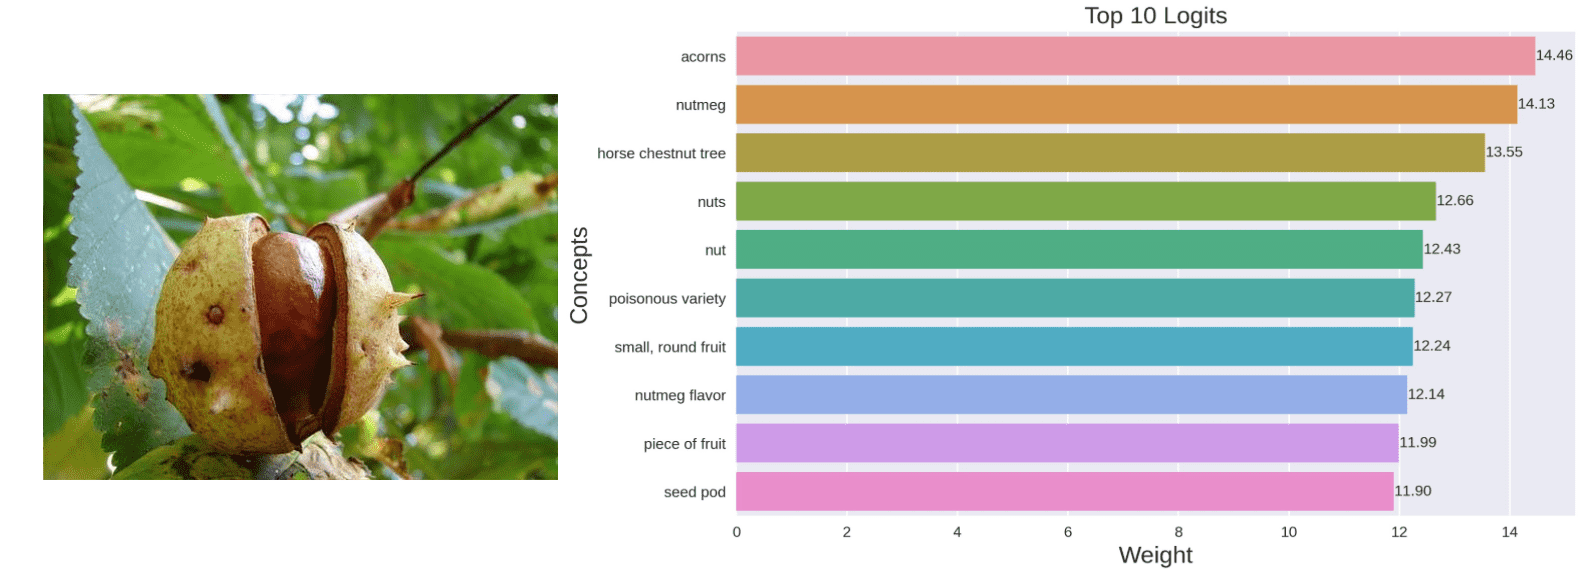
\includegraphics[width=0.75\linewidth]{./figures/contr_im_5-compressed.png}
    % \caption{Концепты, извлекаемые с помощью Contrastive-CBM.}
    \\
    (d) Концепты, извлекаемые с помощью Contrastive-CBM.
    % \label{fig:contr_im_5}
    \end{subfigure}
    \caption{Концепты, извлекаемые с помощью моделей, обученных на Places365.}
    \label{fig:concepts_5}
\end{figure}

\begin{figure}[h] %ht!
\centering
   \begin{subfigure}%[b]%{3.5cm}
     \centering
    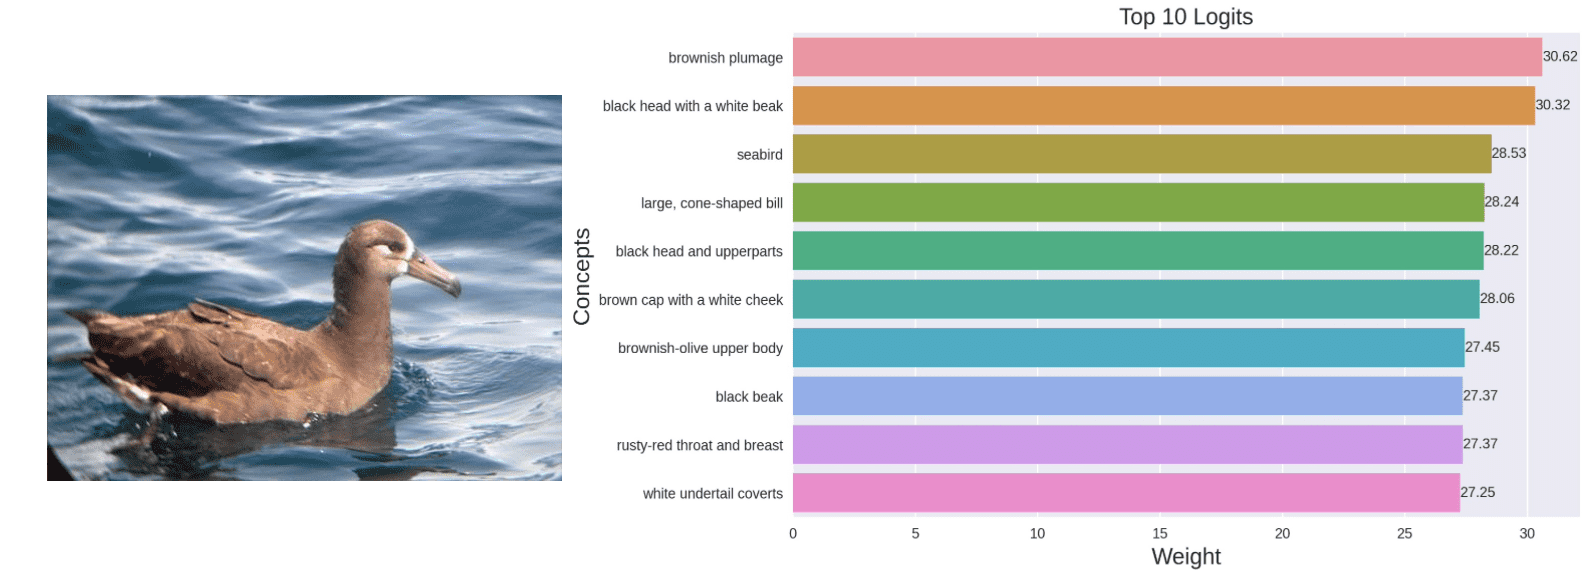
\includegraphics[width=0.75\linewidth]{./figures/clip_im_6-compressed.png}
    % \caption{Концепты, извлекаемые с помощью CLIP.}
    \\
    (a) Концепты, извлекаемые с помощью CLIP.
    % \label{fig:clip_im_6}
    \end{subfigure}
    \begin{subfigure}%[b]%{3.5cm}
    \centering
      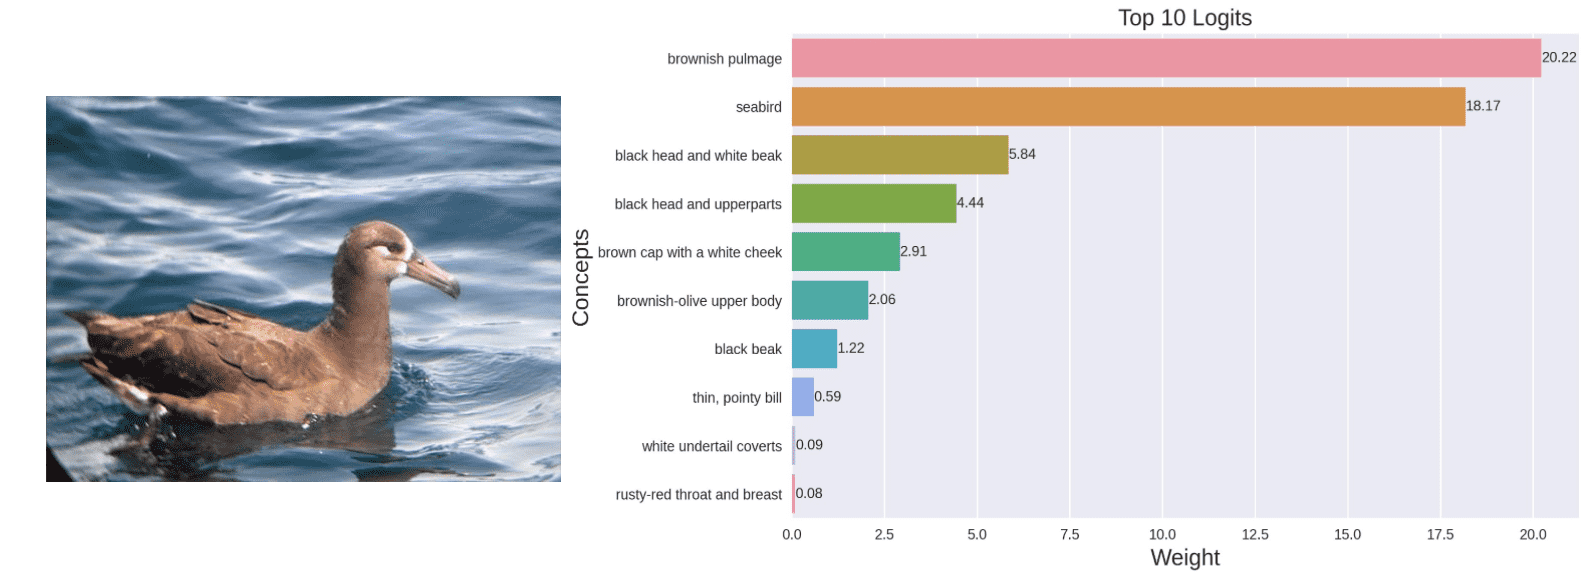
\includegraphics[width=0.75\linewidth]{./figures/sparse_im_6-compressed.png}
    % \caption{Концепты, извлекаемые с помощью Sparse-CBM.}
    \\
    (b) Концепты, извлекаемые с помощью Sparse-CBM.
    % \label{fig:sparse_im_6}
    \end{subfigure}
    \begin{subfigure}%[b]%{3.5cm}
     \centering
  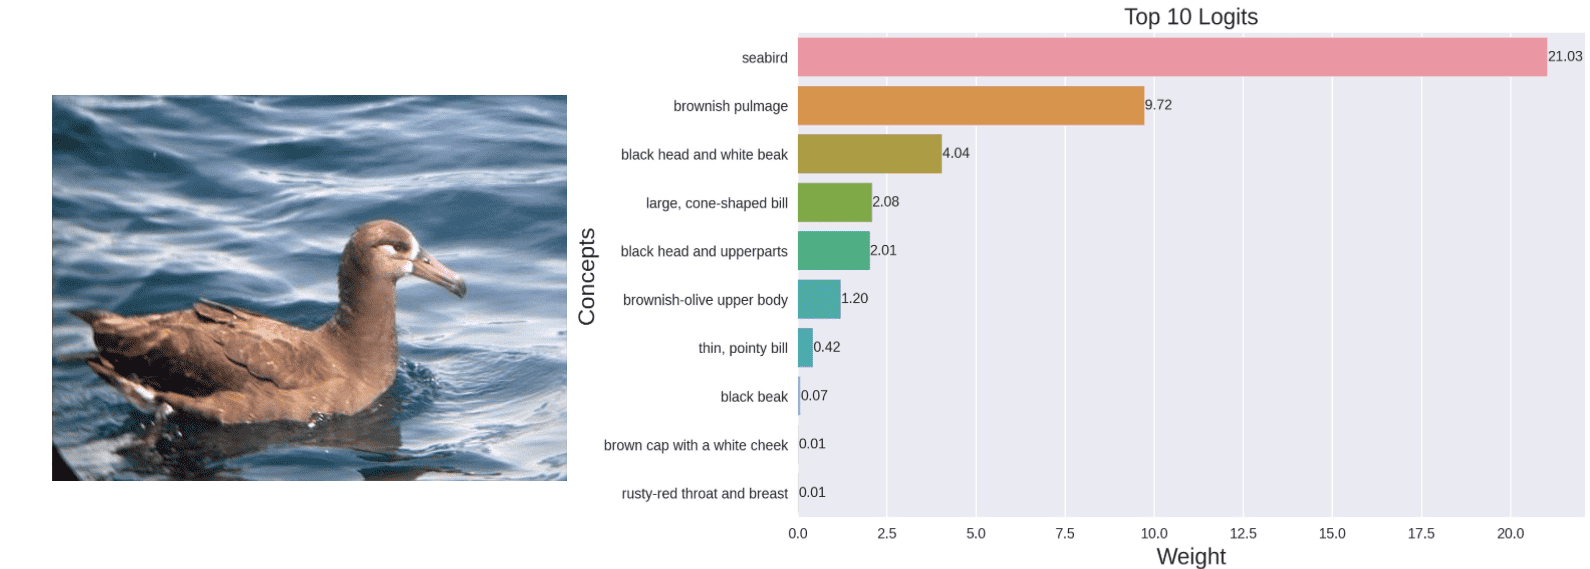
\includegraphics[width=0.75\linewidth]{./figures/l1_im_6-compressed.png}
    % \caption{Концепты, извлекаемые с помощью $\ell_1$-CBM.}
    \\
    (c) Концепты, извлекаемые с помощью $\ell_1$-CBM.
    % \label{fig:l1_im_6}
    \end{subfigure}
        \begin{subfigure}%[b]%{3.5cm}
     \centering
  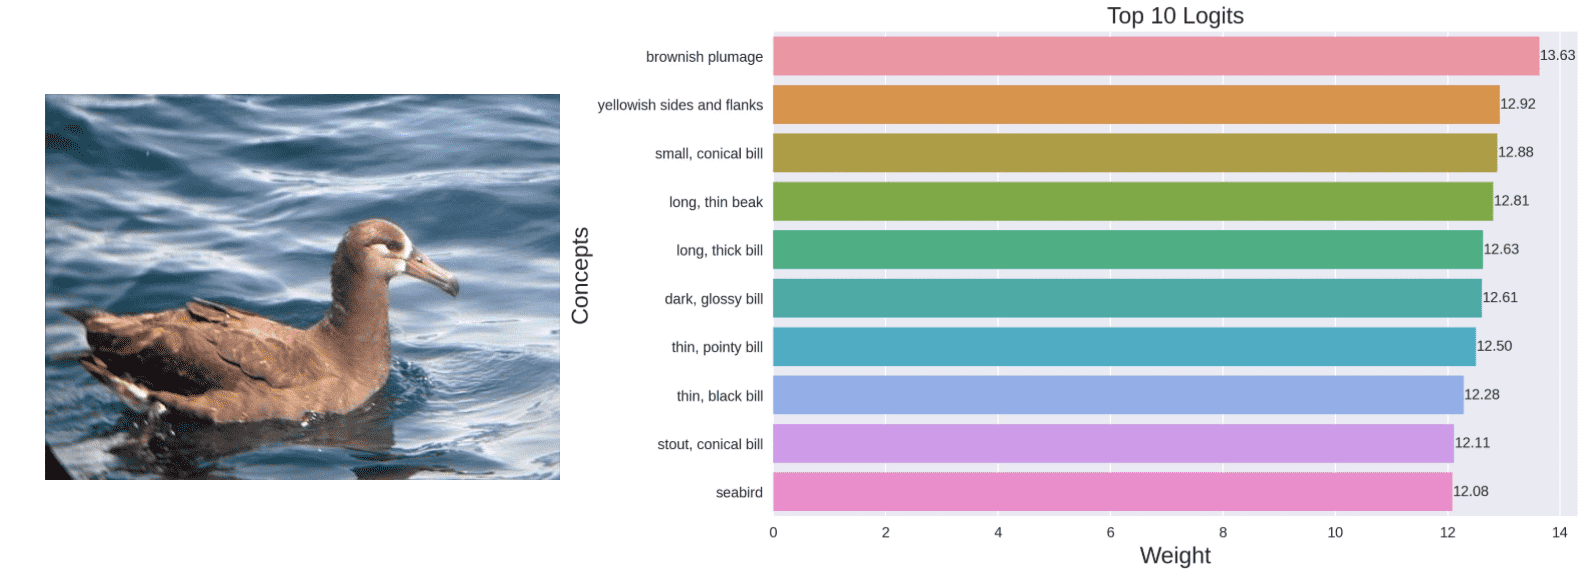
\includegraphics[width=0.75\linewidth]{./figures/contr_im_6-compressed.png}
    % \caption{Концепты, извлекаемые с помощью Contrastive-CBM.}
    \\
    (d) Концепты, извлекаемые с помощью Contrastive-CBM.
    % \label{fig:contr_im_6}
    \end{subfigure}
    \caption{Концепты, извлекаемые с помощью моделей, обученных на CUB200.}
    \label{fig:concepts_6}
\end{figure}

\subsection{Sparse-CBM ошибки}
\label{sec:sparse_confusion}
Вместе с итоговыми результатами классификации мы приводим матрицу путаницы лучшей Sparse-CBM, обученной на наборе данных CUB200, которая достигает 80,02\% точности в \cref{fig:cub_conf_matrix}. Следует заметить, что наиболее значительные ошибки модели закладываются в последней части меток. Сюда входят несколько схожих классов, таких как "черношапочный вирео", "синеголовый вирео", "филадельфийский вирео", "красноглазый вирео", "певчий вирео", "белоглазый вирео" и "желтоголовый вирео". В целом, в таких разнообразных наборах данных, как CUB200, представлено множество схожих классов, поэтому имеет смысл рассмотреть возможность выделения понятий и подчеркнуть их различия между такими классами, как "красноглазый вирео" и "белоглазый вирео".

\begin{figure}[t]%{l}{0.25\textwidth}
\begin{center}
\centerline{
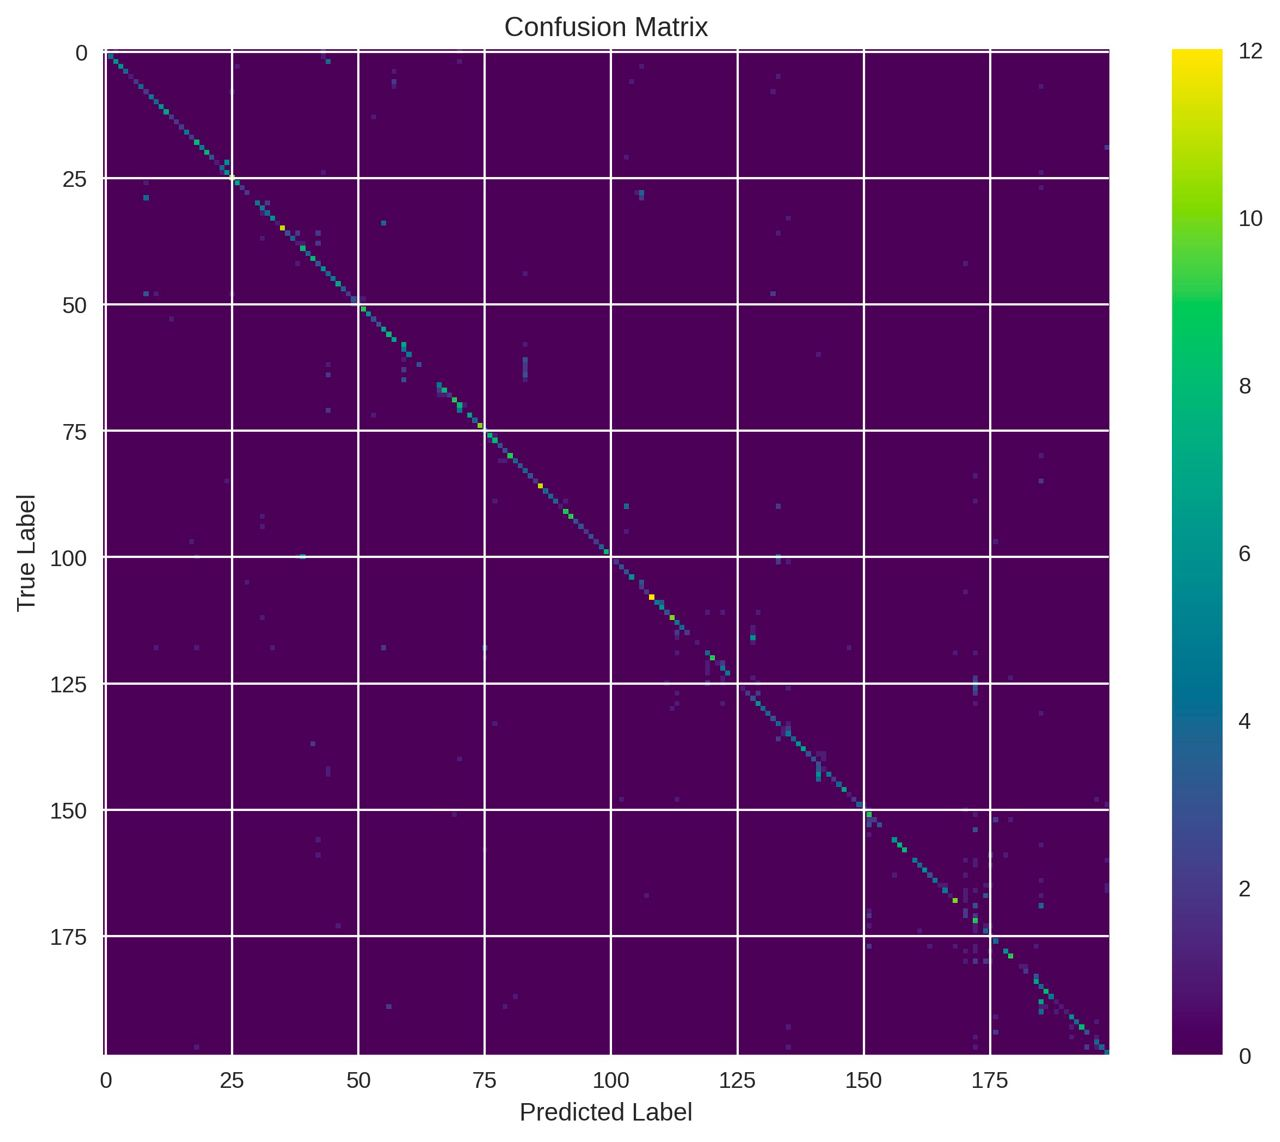
\includegraphics[width=0.6\columnwidth]{./figures/cub_conf_matrix.jpg}}
\caption{Матрица ошибок Sparse-CBM на наборе данных CUB200.}
\label{fig:cub_conf_matrix}
\end{center}
\end{figure}